\documentclass[a4j,11pt,twocolumn,openany]{jsbook}
\usepackage[dvipdfmx]{color}
\usepackage[dvipdfmx]{graphicx}
\usepackage{wrapfig}
\usepackage{float}
\usepackage[deluxe]{otf}
\usepackage[haranoaji]{pxchfon}
\usepackage{longtable}
\usepackage{ulem}
\usepackage{ascmac}
\usepackage{multicol}
\usepackage[Bjornstrup]{fncychap}
\usepackage{titlesec}
\usepackage{picture}
\usepackage{okumacro}
\usepackage{textcomp}
\usepackage{enumitem} 
%\topmargin-2.3cm\advance\textwidth3.0cm
%\oddsidemargin-.5cm\advance\textheight-.5cm
\definecolor{teal}{RGB}{128,128,128}

\setlength{\textwidth}{160truemm}      % テキスト幅: 160mm
\setlength{\fullwidth}{\textwidth}     % ページ全体の幅
\setlength{\oddsidemargin}{0mm}   % 左余白
\setlength{\topmargin}{0mm}       % 上余白
\setlength{\textheight}{230truemm}     % テキスト高さ: 297-(30+30)=237mm
%%%
%見出しの設定 section                                                                                                                                                                                                                                                                                                                                                              
\titleformat{\section}[block]
{}{}{0pt}
{
  \colorbox{teal}{\begin{picture}(0,10)\end{picture}}
  \hspace{0pt}
  \normalfont \large\bfseries \thesection \hangindent=3.5zw % ぶら下げインデント3.5文字
  \hspace{0pt}
}
[
\begin{picture}(100,0)
  \put(4,14){\color{teal}\line(1,0){150}}
\end{picture}
\\
\vspace{-30pt}
]
%%%
%%%% 目次の設定
%\makeatletter
%\renewcommand*{\l@section} {\@dottedtocline{1}{1zw}{4zw}}
%\makeatother
%%%%


\title{学芸員のひみつ道具}% 文書のタイトル
\date{\today}
\author{北海道博物館協会学芸職員部会}              % 著者

%------------------------------
\begin{document}
%\maketitle
\frontmatter % 序文の開始

\tableofcontents

%%%%
\mainmatter
%%%%%%
\chapter{特別講演「ユベオッ(続縄文)時代の概説」記録}

\begin{description}
\item[日 時]2021年(土)13時30分\CID{00665}15時00分
\item[発表者]佐藤剛氏(和人の研究者・公益財団法人北海道埋蔵文化財センター)
\item[公開方法]Zoomによるオンライン配信
\item[参加者]26名
\end{description}

%%%%
\section{ヤウンモシ\CID{16249}とは}
北海道は様々な意味を持ちすぎている。行政的な区分であり、地理的な区域であり、歴史的には国郡制の回復を目指した明治政府の意図なども含まれ、多義的な呼称と考える。「アイヌモシ\CID{16249}」という表現もあり得るが、神の世界「カムイモシ\CID{16249}」の対義語になる「人間の世界」とでもいうべき概念であり、実態的な地理区分には適さないと考えている。そのため、本稿では北海道島を指す地理的区分として「ヤウンモシ\CID{16249}」島を使用する。

%%%%
\section{研究者としての「名乗り」}
アイヌ民族出自の研究者やそれを背景として活動する人々は、少数者として「アイヌ民族」であることを表明するかしないかの選択を迫られる。一方、多数者である和人は自身の由来を表明すること自体を思いにのせることはないように見受けられる。この島について言及するときには多数者としての位置づけに自覚的である必要があるのではないか。「アイヌ」(アイヌ民族)と等置する「和人」(和民族)の表明は、具体的に文字として、言葉として表現する必要がある。そのような考えから「和人の研究者」として発表させていただいている。みなさんと共有したい。

%%%%
\section{続縄文文化研究}
続縄文文化研究の到達点は2010年の『北海道考古学』誌上において、熊木敏朗氏によって整理されている。

その後の土器研究では鈴木信氏と大坂拓氏は江別太式と後北式を細分した型式について検討を行った。
鈴木氏と大坂氏では、「型式」と「細分した型式」の認識に差異がある。「細分した型式」が高じてしまうと研究者間での認識に齟齬が生じてしまう。対話が必要だろう。

後北式の文様は擬縄貼付文などで構成されるものと主に帯状縄文で構成される「帯縄文系」がある。私は鈴木信氏と同様に江別太\ajRoman{3}層の各文化層をそのまま編年に用いることはできないと考える。大坂氏のように「江別太式の全てを後北式に含める」との結論は承知できない。江別太式と後北式は混在しないため、型式的な独立性が高いと言える。これは高橋正勝氏(1984)の意図でもあると考える。

%%%%
\section{弥生文化と恵山式}

恵山式期は掘り込みの明確な竪穴住居と近接する墓域、盛土遺構などの定住的な要素がみられ、弥生文化・弥生社会が展開していた。

続縄文文化は縄文晩期に続くこの島の文化であり、続縄文文化初頭の道南部には道央部と共通性の高い土器群にくわえ、遊動的な要素が強くみられる。その後、下添山式・恵山式の時期に弥生文化化する。その後、後北B式、C{\footnotesize 1}式の頃に再び続縄文文化化すると考える。

続縄文初頭土器群は在地縄文晩期社会の主体的な選択と考えられ、用いる道具を少数に厳選した、移動生活を中心とする遊動的な集落社会と考えられる。続縄文社会は総じて遊動的な集落社会の文化・時代である。後続する前期擦文式土器様式を用いた文化は作り付け竃をもち、定住的な集落を基盤とする社会と位置づけられる。

%%%%
\section{「続縄文時代」呼称}

古墳時代や弥生時代などと等置する考え方からは「ユベオッ(続縄文)時代」とすることが必要である。横山英介氏らの「続縄文時代」の時代区分に疑義を示す立場もあるが、日本列島における固有な島としての地域の歴史の解明には必要な時代区分だと考えている。

%%%%
\section{質疑}

\subparagraph{Sさん}遊動社会をもって続縄文の指標とする概念は面白いと思う。しかし、それは文化の説明であって、共存する諸型式の常時的組み合わせとしての文化の定義にはならないのではないか。近藤義郎さんが述べられているとおり、特徴的な遺物の出現をもって画期を設定することから、遊動社会というだけでは画期を設定することはできないと考える。続縄文文化を遊動社会として理解する考え方はわかったが、考古学における時代と文化の概念にのっとった説明をしなければならないと感じた。
また、恵山文化を定住社会と考え、続縄文文化から外すという説明は理解したが、だからといって、弥生文化の中に入れることはなかなか理解できることではないのではないか。弥生文化は灌漑稲作の出現をもって画期を設定している研究者が多い。弥生的な部分があることは理解しても、弥生文化に含めることは難しいと考えている。
\subparagraph{佐藤}私は考古学は歴史学の一分野と考えており、弥生文化、古墳文化の捉え方は様々あるが、ユベオッ文化は先行研究と本稿により説明されてきていると考える。弥生文化について灌漑稲作を指標とすることにはいくつか異論も出ている。弥生文化地域においても海洋民などは稲作をしていないと思う。時代区分も、これまでの研究とそれを特徴的に示す土器様式の検討から区分しており、ユベオッ時代を区分することは可能だと考える。考古学的な文化の定義は今後も検討していく必要がある。歴史的にアイヌ民族を先住民族と考えた時、アイヌ文化期とか続縄文文化のような問題のある時期区分、時代区分ではないものを用語として使用してきた。私はその点が違うと考える。
\subparagraph{Sさん}時代と文化を区分した議論が必要。東北の弥生文化も時代区分について指標が明確に示されたほうが良いと思う。
\subparagraph{Sさん}横山(浩一)さんの型式はタイプのことを述べている。
\subparagraph{司会}横山さんの型式の理解についてもう一度説明をお願いしたい。
\subparagraph{佐藤}私の発表は横山さんの型式論をベースに考えている。型式を細分していくと再現性がなくなってしまうということを述べたかった。
\subparagraph{Sさん}大坂さんと鈴木さんの議論が噛み合わないのは、そうした型式理解に齟齬があるからなのだろうと思う。
\subparagraph{Tさん}続縄文の前半と後半の違いが大きく、縄文と続縄文との間の隔たりよりも大きいようにも思える。縄文と続縄文の内部の差異、また、本州の弥生とどう区分できるのかお聞かせ願いたい。
\subparagraph{佐藤}縄文は定住的な土器群、続縄文は移動しながら生活する土器群と区分することができる。細別器種の構成が少ない続縄文の土器様式は遊動的な生活に適応しているものと考える。前期擦文式土器様式は6世紀末に成立したと考えるが、同時期の東北地方の土器様式と比較すると、細別器種が少ない。甕や杯はあるが、その量は少ないと言える。6世紀末の東北地方では稲作を行う地域がほとんどであり、定住的で稲作を行う律令社会と定住的でありながら狩猟漁労採集をする擦文社会に分けられると考える。続縄文の最後の段階は、縄文がつく土器までを続縄文と区分する方もいるが、細別器種にもとづいて区分する立場から、縄文がない段階でも細別器種構成が似た段階がある。
\subparagraph{Tさん}恵山文化は器種が少ないのか。
\subparagraph{佐藤}恵山文化は細別器種が多いと捉える。
\subparagraph{Tさん}だとすると、恵山文化が続縄文文化に属しているのはどのように捉えれば良いのか。
\subparagraph{佐藤}私は恵山文化は続縄文の文化に含めて考えていない。
\subparagraph{Tさん}本州の弥生文化が稲作の有無をもって弥生文化の区分を考えているので、そうなると恵山文化の位置づけが難しくなる。続縄文でも弥生でもない文化ということになるのかという感想を持った。
\subparagraph{佐藤}なぜ本州島の区分をそのまま適用しなければならないのかという疑問はあるが、適用したとしても恵山文化は弥生文化の海洋民として捉えて良いと思っている。
\subparagraph{司会}恵山文化が海洋民だということは、土器からわかることではなく、その他の遺物構成から判断しているということか。
\subparagraph{佐藤}弥生文化として土器様式でも区分できると考えるが、骨角器などの検討も先行研究があり、海洋民と考えている。恵山文化の総体は道南部にしかない。道央部には恵山式土器は客体的にしか入らない。縄文晩期の大洞C1式の土器は道央部まで広がっている。その時に社会の変化がどのように起きているのかはさほど検討されずに、単に亀ヶ岡文化の広がりとして捉えられてきた。恵山文化の場合は、盛土遺構や貝塚や掘り込みのしっかりした竪穴住居などは定住的な集落社会を示しており、稲作を行っていないだけで、同時期の本州北部の弥生文化のもつ遺構・遺物群と変わらない。
\subparagraph{Tさん}本日の成果はぜひ論文として発表して、全体として共有していただきたい。そうしなければ、議論が深まらない。
\subparagraph{佐藤}今回の発表は概説のため論考としてまとめきれていないので、すぐには難しいが努力する。それまでは本稿を参照していただきたい。
\subparagraph{Tさん}博物館学芸員として、続縄文やアイヌ民族の解説で苦慮することがあり、参考になった。
\subparagraph{司会}次の12月には本講演と同じく続縄文文化をテーマとした情報交換会を予定している。その際には何らかの形で資料集を公開したい。佐藤さんには講演内容を論文化していただくことを事務局からもお願いしたい。

%%%%
\noindent
\hrulefill

佐藤氏講演資料を含む誌上報告資料は下記のURLからダウンロードできます。

https://ishiijunpei.github.io/dkouko2020/

\begin{flushright}
	(石井淳平)
\end{flushright}

%%%%
\chapter{研究ノート\\岩手県野田村の弥生小型壺と北海道江別市の続縄文小型壺}

\section{はじめに}
筆者は2016\CID{00665}17年に公益財団法人岩手県文化振興財団埋蔵文化財センター(以下、岩埋文)に所属し、2016年に岩手県野田村上代川遺跡(岩手埋文 2020)の発掘調査に携わった。遺跡は中世の製鉄遺構が主体だが、弥生中期\CID{00665}後期を主に弥生土器も出土した(同 p.168-173)。その中に小型壺(図2同 p.200-59)があった。そして、これに類した壺が北海道江別市旧豊平川河畔遺跡(図3江別市1983 p.18-6,石川 2005 p.19-2)にあった。岩手県野田村と江別市の間に位置する道南で活動する南北海道考古学情報交換会会誌に紹介し、皆様から御教示いただきたい。

\section{野田村上代川遺跡の小型壺}\label{nodamura}
竪穴住居SI06埋土出土。この埋土は弥生中期後半・川岸場式を主として後期・赤穴式までの土器が出土する。小型壺は頸部に穿孔が一か所ある。その頸部には横走沈線が巡る。無紋地に二本一組の沈線で器表面のほぼ全面に施文する。肩と底部際には鋸歯状文が巡る。底部は上げ底気味、器壁厚さは比較的一定で、口唇断面形状はすぼまる。胴部は弧状の沈線が方形区画内に収まった文様が横に連続する構成である。時期は、遺跡報告書の分類記号(岩埋文 2020p.167)で\ajRoman{5}群3類A(本文:同 p.162-163,図:同 p.169\footnote{
	掲載表(岩埋文2020 p.371)の\ajRoman{5}群4類は誤り
})である。\ajRoman{5}群3類とは、弥生中葉は川岸場式の頃、Aは恵山式や田舎館式といった、より北からの影響がある土器群を指す。大きさは、口径約4.8cm、底径5.0cm、、高さ12.0cmで、頸部径は4.6cm、胴部径は9.2cmである。

\begin{figure}[ht]
	\centering
	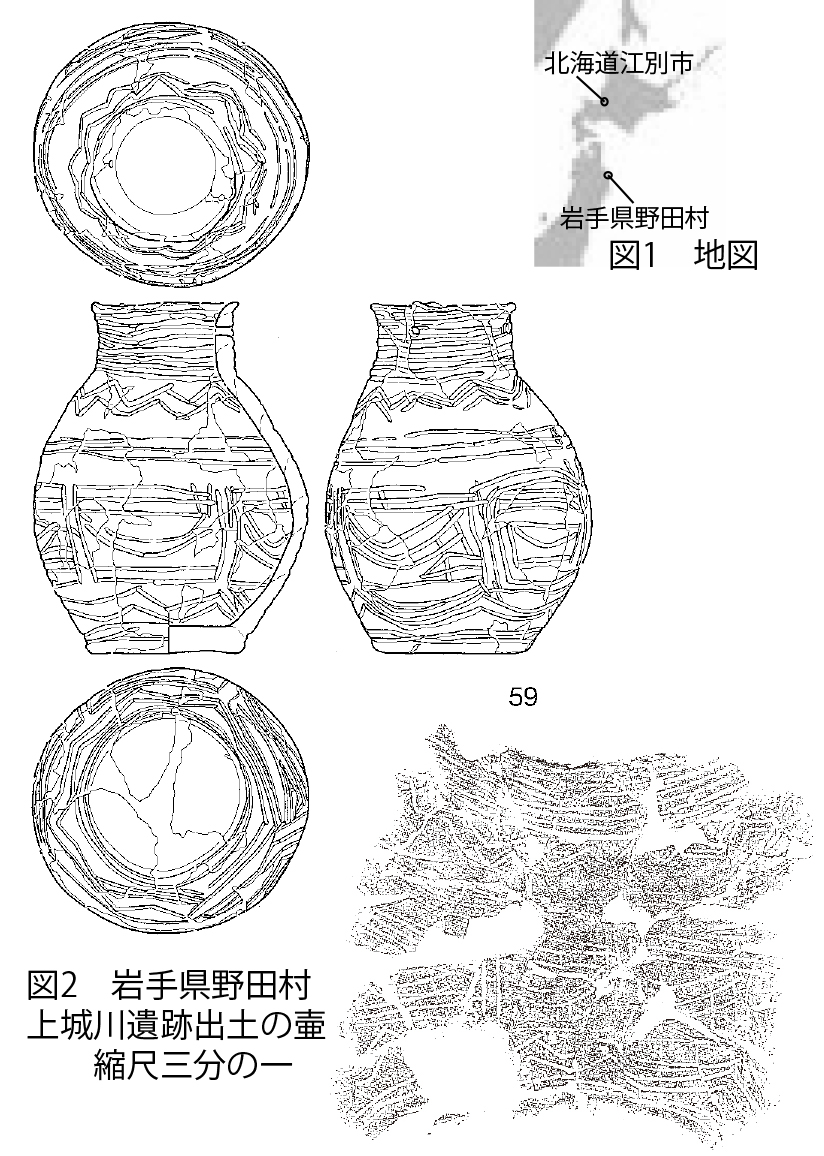
\includegraphics[width=\linewidth]{fig/03_Otaishi/01_otaishi.jpg}
	\label{}
	\vspace{-2\baselineskip}
\end{figure}

%%%%
\section{江別市旧豊平川河畔遺跡の小型壺}
遺跡は旧豊平川(世田豊平川)を見下ろす台地の縁にあり、江別チャシも同じ台地上にある。壺は墓18から出土した(図3)。図3aは再実測と拓本(石川2005)、図3bは当初の報告図(江別市1983)である。図2で示したものと同様、頸部の一か所に穿孔があり、こちらは二つの穴で一組となる。頸部には横走沈線が巡るが穿孔部分より上、口唇際は無紋となる。縄文地に三本一組の沈線で施文し、肩部に鋸歯状文が巡る。底部は上げ底気味で、器壁厚さはほぼ一定、口唇断面形状はすぼまる。胴部は弧線文が横方向へ並ぶ。うろこ状に近いが一部は不規則である。胴部下・底部際は沈線文が無く縄文のみである。大きさは口径4.2cm、底径4.6cm、高さ13.6cmで、頸部径は3.8cm、胴部最大径は9.8cmである。

\begin{figure*}[ht]
	\centering
	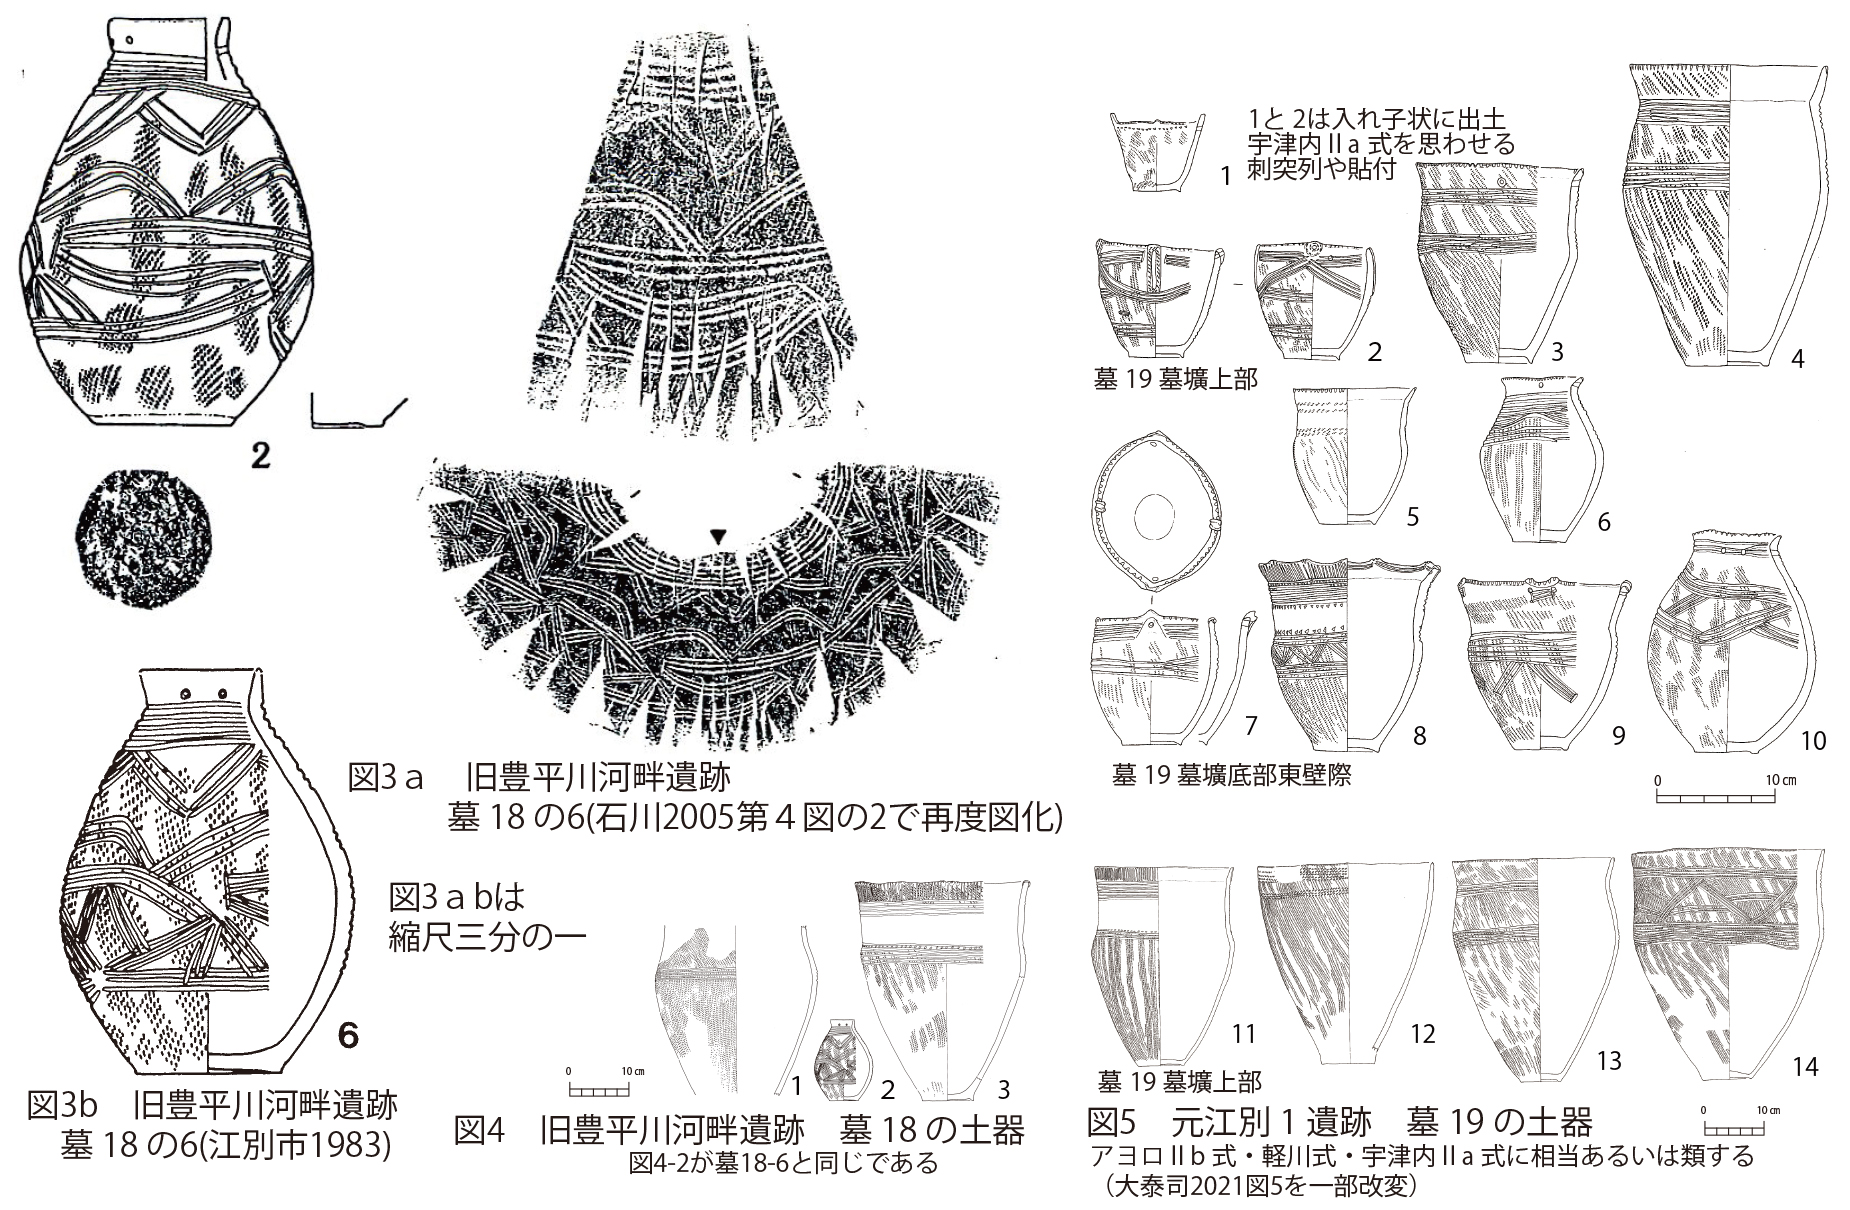
\includegraphics[width=160truemm]{fig/03_Otaishi/02_otaishi.jpg}
	\label{}
	\vspace{-1\baselineskip}
\end{figure*}

\begin{figure*}[ht]
	\centering
	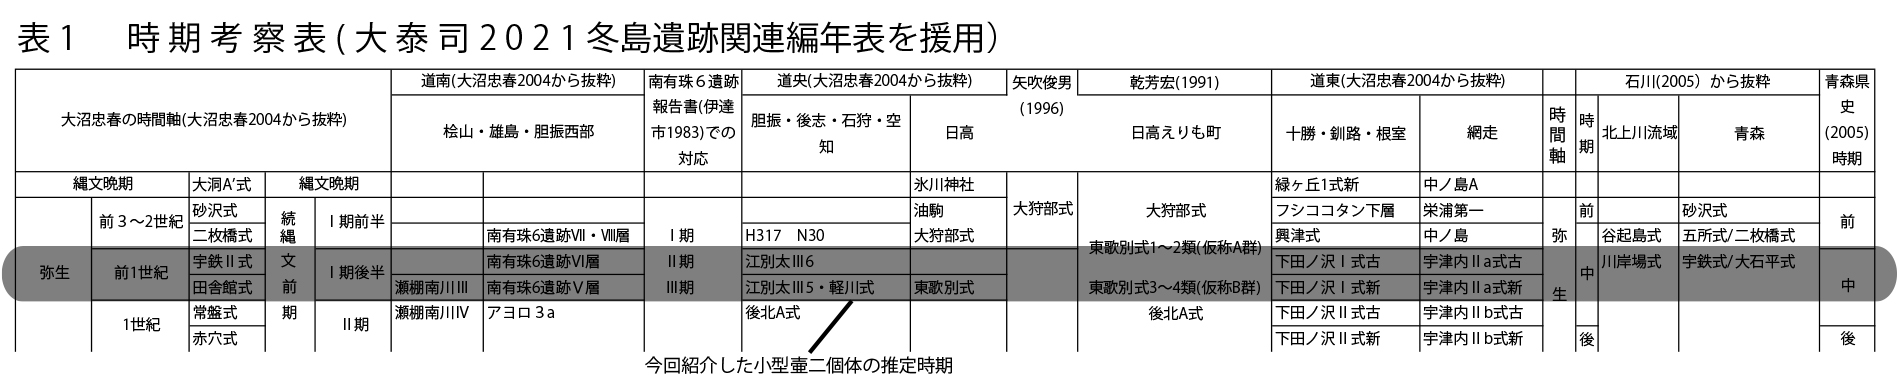
\includegraphics[width=160truemm]{fig/03_Otaishi/03_otaishi.jpg}
	\label{}
	\vspace{-1\baselineskip}
\end{figure*}

上代川遺跡出土のものと比較すると、高さに比べて横幅が若干狭く全体的に細めである。また無紋に対して縄文地紋である。無紋帯が頸部から口唇にかけて巡り、底部際も地紋のみである。器壁の厚みは一定で、上げ底気味の底部と口唇断面の形状に類似点がある。他にも、二本と三本の違いはあるが複数本の沈線で施文する点と、頸部に一単位の穿孔があることが挙げられる。

%%%%
\section{壺の時期}
墓18出土土器の時期を考察する。豊平川河畔遺跡墓18出土土器(図4-1\CID{00665}3)は、出土地点から南西に約400m離れた元江別1遺跡墓19出土土器に似る。墓19出土14個体の復元土器には二本ないし三本一組の沈線施文を持つ個体が目立つ(大泰司2021 p.11)。

豊平川河畔遺跡墓18(図4)と元江別1遺跡墓19(図5)の出土土器群を比較すると、墓18図4-1は縄文地紋で胴部最大径部分の横走沈線が、墓19図5-3・13と似る。小型壺図4-2は図3と同一で、一単位の穿孔と胴部文様構成、口唇際の無紋帯と底部際が縄文地紋のみで沈線文が無い点が図5-6・10に似る。図4-3は頸部に幅広い無紋帯があり、その上下に横走沈線が巡り、帯の下に刺突列が横方向に並ぶ点、そして、口唇部に縦方向の短沈線が横方向に連続して並ぶ点、そして器形が図5-11と似ている。よって両群は時期的に近いと考える。両群を様似町冬島遺跡出土土器の検討(大泰司2021 p.15)で作成した表1において、網掛けで示した時期に位置すると考えたい。その結果、川岸場式並行の可能性が高く、上代川遺跡と豊平川河畔遺跡の小型壺も同様に近い時期の土器と考えた。
上代川遺跡出土弥生土器は川岸場式の頃を\ajRoman{5}群3類として、そのうち文様要素から、田舎館式ひいては恵山式の影響が考えられるものをAとしたことは\ref{nodamura}項で触れたが。まとまりは三つあり、残り二つのうちBは北上川沿いの土器型式・川岸場式、Cは馬淵川・新井田川流域・八戸市域ないし野田村の在地的な特徴を持つ土器(岩埋文2020 p.167)である。

Aとした今回の小型壺が江別市の小型壺と「類同」とまではいかないが、類似点があったことを記した。今後も検討を続けたい。

江別市元江別1遺跡墓19出土土器と、様似町冬島遺跡出土土器に類似点があったという内容の文章(大泰司2021p.10-11)を今回、引用した。この様似町と野田村とは人の行き来が盛んで、1998年に友好町村を締結した。この人々の動きは、流れの強い津軽暖流を避けた結果なのであろうか。

上代川遺跡では北田勲氏の采配の元、作業に没頭できた。土器整理は石川日出志先生のお力で乗り切ることができた。江別市では佐藤一志氏に便宜を図っていただいた。そして、佐藤由紀男先生、大坂拓氏から御助言をいただいた。記して謝意を表したい。
\vspace{1\baselineskip}

%%%%
\subsection*{参考文献}

{\small
	\hangindent=1zw
	\noindent
	石川日出志 2005『関東・東北弥生土器と北海道続縄文土器の広域編年』
	
	\hangindent=1zw
	\noindent
	公益財団法人岩手県文化振興財団埋蔵文化財センター 2020『上代川遺跡発掘調査報告書』岩手県文化振興事業団埋蔵文化財調査報告書第713集
	
	\hangindent=1zw
	\noindent
	江別市教育委員会 1983『町村農場1・七丁目沢7・旧豊平川河畔―江別チャシ―・後藤・大麻3』江別市文化財調査報告書\ajRoman{10}\ajRoman{7}
	
	\hangindent=1zw
	\noindent
	江別市教育委員会 1981『元江別遺跡群 後藤遺跡 旧豊平川河畔遺跡 元江別1遺跡 元江別2遺跡 元江別5遺跡 元江別10遺跡 元江別11遺跡』江別市文化財調査報告書\ajRoman{10}\ajRoman{3}
	
	\hangindent=1zw
	\noindent
	大泰司統 2021「冬島遺跡の特徴的な土器」『様似郷土館紀要 3号』
	
}

\begin{flushright}
	大泰司 統\\((公財)北海道埋蔵文化財センター)
\end{flushright}


%%%%
\chapter{研究ノート\\空中写真を利用した地形測量による遺跡探査の試み}

\section{はじめに}
今金町教育委員会では2020年度から文化財の総合的な把握調査を行っており、既知の文化財以外に所在地や内容が未確認のものについても調査対象とし、文献史料等を参照しながらその把握に努めている。

そうした史料の中でも重要なのが、幕末の1857年(安政4)に当地域を貫流する後志利別川流域を探検した松浦武四郎の文書史料(松浦/秋葉1982)である。以下、便宜上これを「松浦史料」と呼ぶ。ここにはすでに地名としては残されていない数多くのアイヌ語地名が記されており、幕末期における当地域の様子を窺い知ることのできる極めて重要な手がかりを提供している。

筆者の一人の宮本はこの中のチャシ地名に注目し、松浦が記した絵図や旅程の記述内容からチャシ跡の現地踏査を行ったが、明確な場所の特定には至らなかった(宮本2018)。今回、戦後アメリカ軍が撮影した航空写真から地形測量する手法を活用し、その成果図をもとに現地調査したところ、踏査を効率化できただけでなく、所在地の特定にも一定の成果を得ることができた。本稿は、こうした空中写真を利用した遺跡探査の実例を紹介し、その有効性について述べる。

%%%%
\section{空中写真を利用した写真測量}

空中写真による写真測量の歴史や原理・方法については本題から外れるため、次に掲げる文献を参照されたい(宮塚1999、木全 1999、佐藤 2009)。

本稿で主に取り上げる空中写真は、アメリカ軍が第二次大戦後に航空機を使用し、日本全土を撮影したものを指す。1947年撮影は縮尺約3万分の1、1948年撮影は縮尺約1.5万の1を中心とした白黒写真である。また、1976年と1977年に国土地理院が縮尺約8千分の1から1万分の1でカラーによる空撮を行った。便宜上、前者を米軍写真、後者を地理院写真と呼称する。

近年、国土地理院は「地図・空中写真閲覧サービス」としてインターネット上で過去に撮影した航空写真を無償提供するようになった。先述の米軍写真も含め、低解像度(400dpi)のものならば無償でダウンロードすることができる。これらの画像は、いずれも写真測量用に60%前後でオーバーラップして撮影されており、図化機を用いなくとも簡易的な方法で立体視することも可能である。

筆者の一人の宮塚は約5年前からこれらの古い航空写真を利用し、北海道内のチャシ跡や竪穴群を図化してきた。終戦後の航空写真は開発行為がまだ進んでおらず、また戦後の荒廃から森林の植林も進んでいないため、特に北海道の遺跡群は撮影時期が早春や晩秋ならば、かなりはっきりと遺跡の痕跡を把握することができることがわかった。使用している図化機はイタリア・シスカム社Stereo Metoric ver.8.0.1である。写真座標は画像の指標を計測し(内部標定)、地形図から絶対座標を取得して(外部標定)、写真座標と絶対座標を相互に標定して、ステレオモデルを作成した。

今回調査対象とした後志利別川流域のチャシ跡について、流域沿いに撮影された米軍写真を主とし、部分的に地理院写真を用い、先述の図化機を使用して立体視し探査した。その結果、主に流域沿いの台地突端部に10カ所以上のチャシ跡特有の壕状地形を発見することができた。以下、これを「可能性地」と呼称する。

%%%%
\section{成果図に基づく現地踏査}
上記の成果図をもとに、可能性地がチャシ跡であるかどうかを確認するため、2021年4月及び同年7月の2回、現地踏査に当たった。すべての可能性地を踏査したわけではないが、その多くが開発行為による地形改変の影響で損壊していたものの、チャシ跡特有の壕状地形の断片的な痕跡を少なくとも3地点で確認することができた。本稿ではそのうちの1つを紹介する。

\begin{figure}[ht]
	\centering
	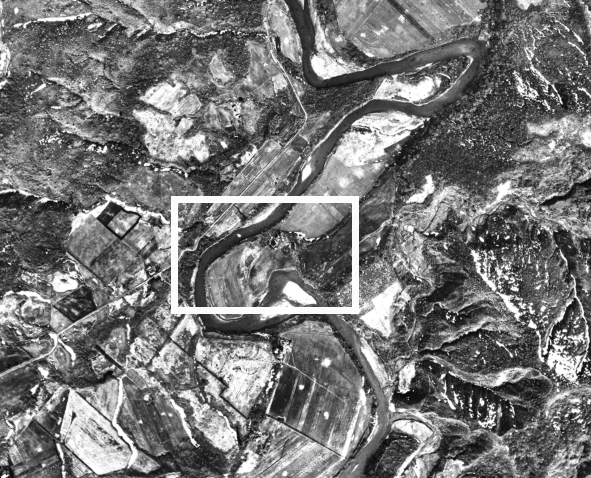
\includegraphics[width=\linewidth]{fig/05_Miyamoto/pic01.pdf}
	\caption{\hangindent=3zw
		1948年米軍撮影のフシコベツ付近(航空写真画像データは国土地理院より転用)}
	\label{miya01pic}
%	\vspace{-\baselineskip}
\end{figure}

\begin{figure}[ht]
	\centering
	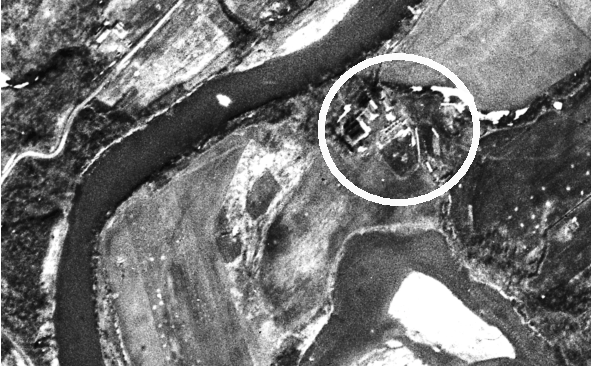
\includegraphics[width=\linewidth]{fig/05_Miyamoto/pic02.pdf}
	\caption{\hangindent=3zw
		図\ref{miya01pic}の矩形で囲った範囲(航空写真画像データは国土地理院より転用)}
	\label{miya02pic}
	\vspace{-\baselineskip}
\end{figure}

\begin{figure}[ht]
	\centering
	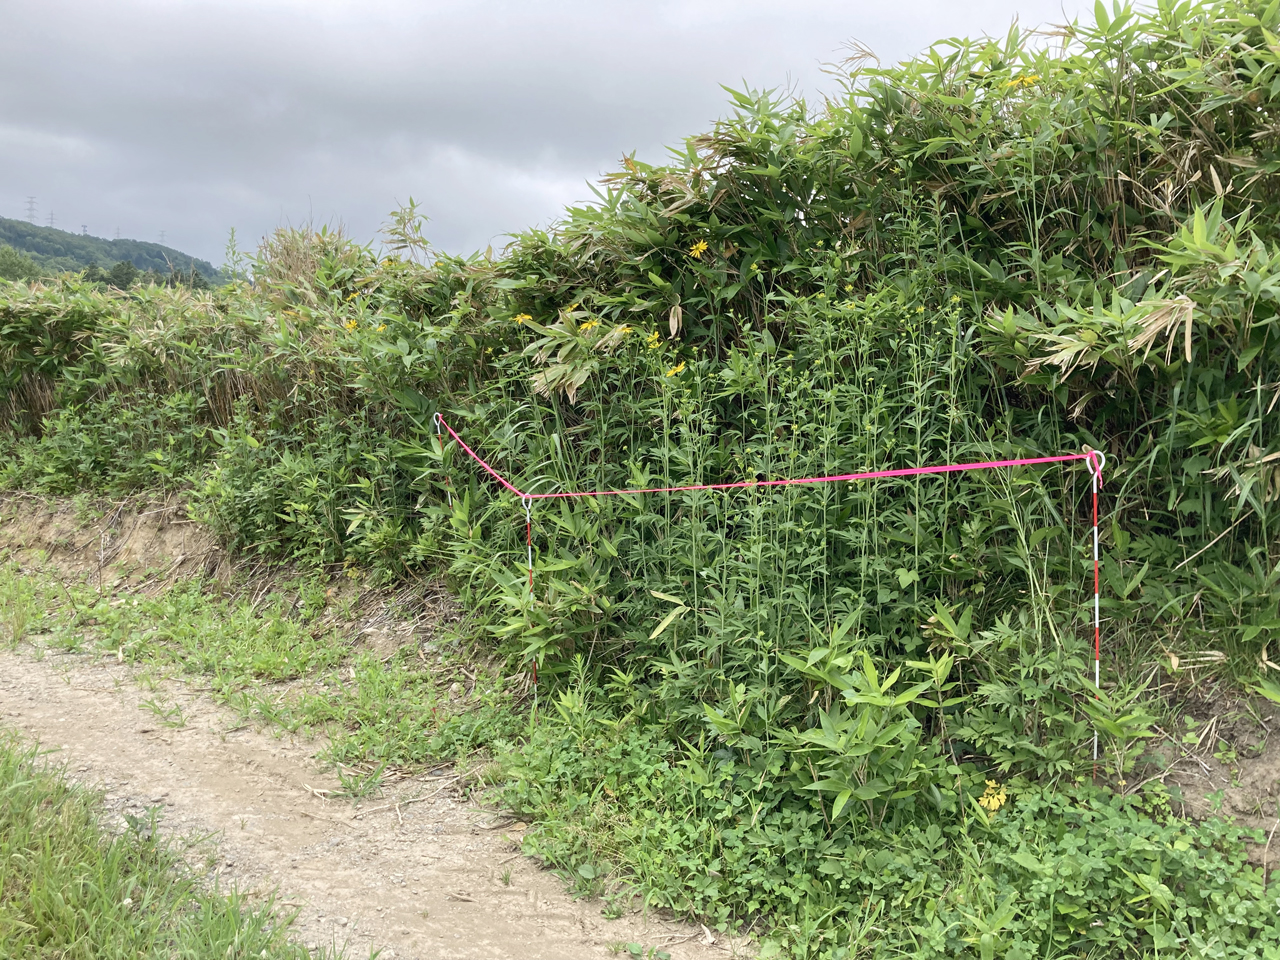
\includegraphics[width=\linewidth]{fig/05_Miyamoto/pic03.jpg}
	\caption{\hangindent=3zw
		法面に見られる壕状地形の痕跡(着色テープ部)}
	\label{miya03pic}
	\vspace{-\baselineskip}
\end{figure}

図\ref{miya01pic}は松浦史料中「フシコベツ」と記される付近を写した米軍写真で、今金町中里地区の後志利別川中流域に当たる。図\ref{miya02pic}はその拡大部で、円で囲んだ範囲を踏査したところ、農地造成によって大半は損壊していたが、台地の西側を削る切通し道路の法面から、チャシ跡の壕と思われる痕跡を発見した(図\ref{miya03pic})。試掘調査による確認を経なければならないが、2重の壕が存在する可能性が高い。

この踏査結果を基に、国土地理院から改めて米軍写真1948年撮影の高精細画像(1200dpi)を購入し、再度図化したものが図\ref{miya01fig}である。

\begin{figure*}[ht]
%	\vspace{-\baselineskip}
	\centering
	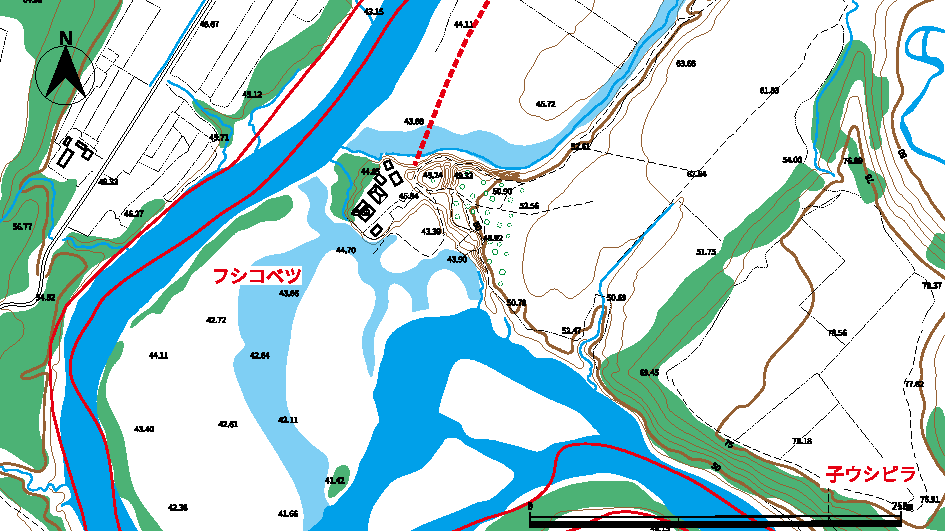
\includegraphics[width=0.9\linewidth]{fig/05_Miyamoto/fig01.pdf}
	\caption{\hangindent=3zw
		米軍写真から作成したフシコベツ付近の地形図(本図は1948年4月28日撮影の米軍写真(国土地理院)を基にStereo Metric Pro ver.8.0.1 を用いて図化したもの。赤線は現河道、赤点線は現農道を示す。)}
	\label{miya01fig}
\end{figure*}

\begin{figure*}[ht]
	\vspace{-0.5\baselineskip}
	\centering
	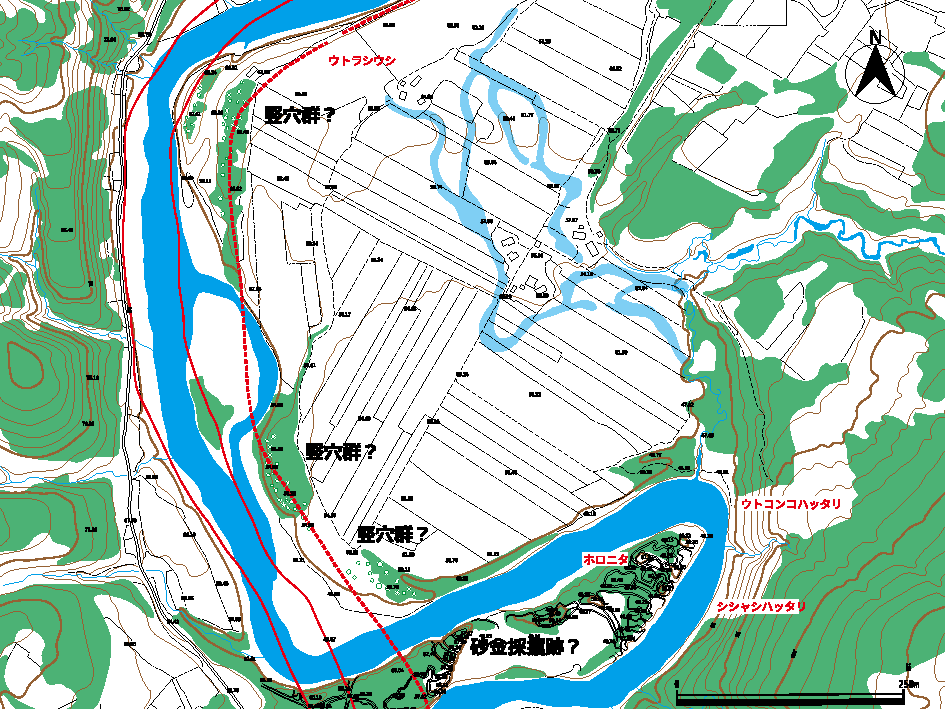
\includegraphics[width=0.9\linewidth]{fig/05_Miyamoto/fig02.pdf}
	\caption{\hangindent=3zw
		図\ref{miya01fig}の北に隣接する区域の地形図(本図は1948年4月28日撮影の米軍写真(国土地理院)を基にStereo Metric Pro ver.8.0.1 を用いて図化したもの。赤線は現河道、赤点線は現農道を示す。)}
	\label{miya02fig}
\end{figure*}

旧河道に囲まれた西向きの舌状台地上にチャシ跡特有の壕状の溝が2条確認できる。また、壕の間とその外側には土塁状の高まりも見て取れる。しかし、先述のように当地点は地形改変が著しく、法面に見られる壕状の痕跡以外は積極的な証拠は認められなかった。

なお、高精細画像の観察中に付随して発見できたのが図3.5である。図3.4の北に隣接する区域で、河川東側に竪穴群のような多数の方形のくぼみ、河川西側には江戸時代の砂金採掘跡に特徴的な水路状遺構が見える(図3.5)。この区域は現地踏査していないので、今後の課題としておきたい。

\section{おわりに}

米軍写真からは約70年前、地理院写真からは約45年前の地形情報が得られ、これらは開発前に存在したであろう遺跡の位置を記録している可能性が高い。これを根拠に、今回見出されたチャシ跡可能性地を踏査した結果、多くは現代の開発行為で削平され、損壊されたものが多かった。しかし、断片的ではあるものの、少なくとも3地点でチャシ特有の地形痕跡を確認することができた。航空写真を立体視し現地に赴くことは、効果的な遺跡踏査の手法として十分活用できることがわかった。

もちろん、今回把握した可能性地については今後試掘調査による確認が必要であり、チャシ跡の存在が確定されたわけではない。

一方、チャシ跡の立地や分布の傾向としては一般に、海岸沿いや河川流域沿いに複数個所、多い地域では20カ所以上連続的に築かれる場合があることが知られている(小林1994)。これを踏まえると、今回認知された後志利別川流域の多数のチャシ跡可能性地についてもその可能性がないとは言えず、むしろその痕跡を指し示している可能性がある。こうして見た場合、松浦が調査した幕末期には、当地域のアイヌの間でもチャシにまつわる伝承がすでに失われており、従って松浦史料にも記載されなかったということも考えられるだろう。

今回の調査を通して、文献史料のみに基づく局所的な踏査に限定することなく、チャシの立地特性の把握や古い写真記録の参照といった多角的、総合的な視点を持つことが重要であることを認識する機会にもなったことを付記しておきたい。
\vspace{1\baselineskip}

\subsection*{参考文献}

{\small 
\hangindent=1zw
\noindent
木全敬蔵 1999「空中写真と考古学」『考古学と自然科学\ajMaru{5} 考古学と調査・情報処理』同成社

\hangindent=1zw
\noindent
小林和夫1994「チャシとアイヌ語地名」『アイヌのチャシとその世界』北海道出版企画センター

\hangindent=1zw
\noindent
佐藤武彦 2009「空中写真測量」『考古調査ハンドブック1 埋蔵文化財調査の基礎テクニック』ニューサイエンス社

\hangindent=1zw
\noindent
松浦武四郎著/秋葉実解読 1982『丁巳東西蝦夷山川地理取調日誌 下』北海道出版企画センター

\hangindent=1zw
\noindent
宮塚義人 1999「遺跡・遺構・遺物の図化情報」『考古学と自然科学\ajMaru{5} 考古学と調査・情報処理』同成社

\hangindent=1zw
\noindent
宮本雅通 2018「今金町におけるアイヌ文化に関する基礎的調査」『和人地とその周辺のアイヌ文化に関する基礎的研究 公益財団法人アイヌ文化振興・研究推進機構 アイヌ関連研究事業研究助成(一般研究)研究概要報告書』

}

\begin{flushright}
	宮本雅通(今金町教育委員会)\\\
	宮塚義人(宮塚文化財研究所)
\end{flushright}


%%%%
\chapter{遺跡見学会報告 南北海道の縄文ツアー}

\begin{description}
	\item [日時] 2021年8月28日(土)10時\CID{00665}12時
	\item [場所] 大船遺跡、大船B遺跡、垣ノ島遺跡
	\item [参加] 20名
\end{description}

世界文化遺産「北海道・北東北の縄文遺跡群」の構成資産となる2つの史跡と函館市南茅部地域で本年度行われている縄文遺跡の発掘調査を見学しました。

最高気温28℃を超える暑い日でしたが、たくさんの方が道南歴史文化振興財団の事務所前に集まってくれました。遺跡へ出発する前に、荻野幸男会員(道南歴史文化振興財団)から大船B遺跡の概要と出土遺物について説明をいただきました。

\begin{figure}[ht]
	\centering
	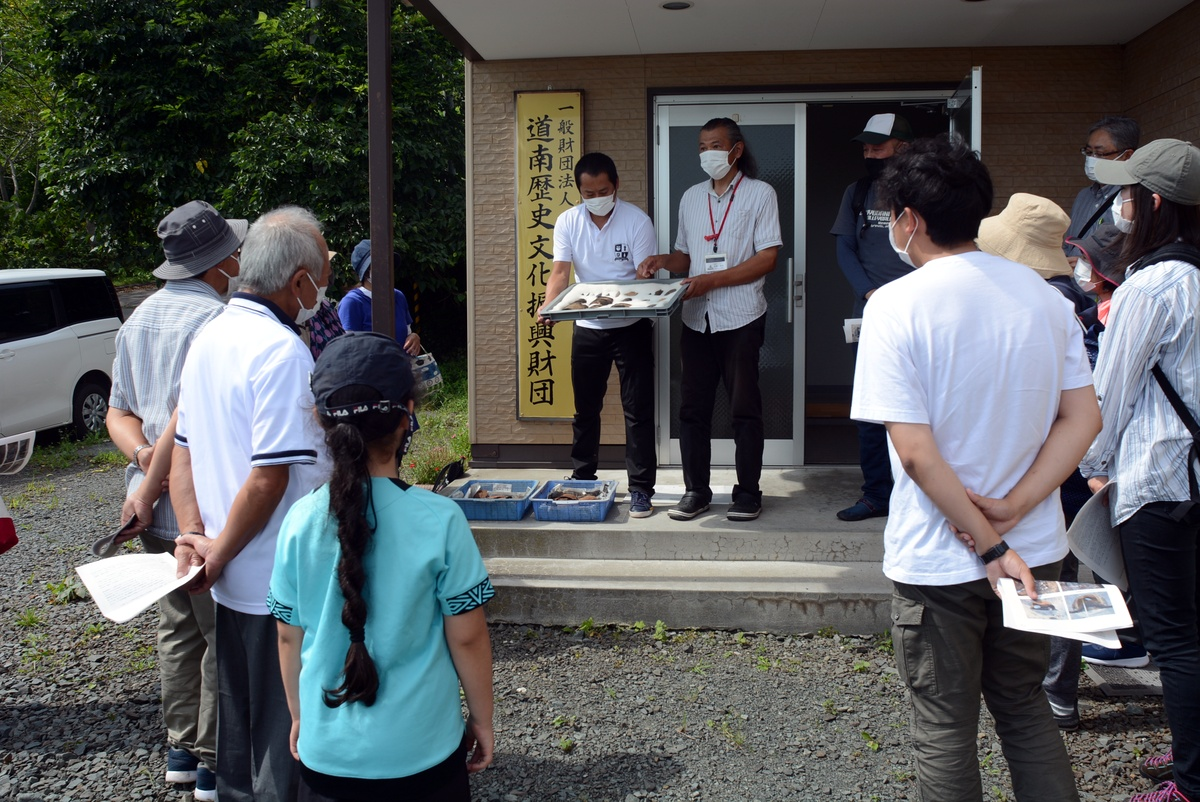
\includegraphics[width=\linewidth]{fig/01_Iseki_kengaku/01_Opening.JPG}
	\caption{大船B遺跡出土遺物の説明をする荻野会員}
	\label{}
\end{figure}

\section{復元竪穴住居が魅力の大船遺跡}

\begin{figure}[ht]
	\centering
	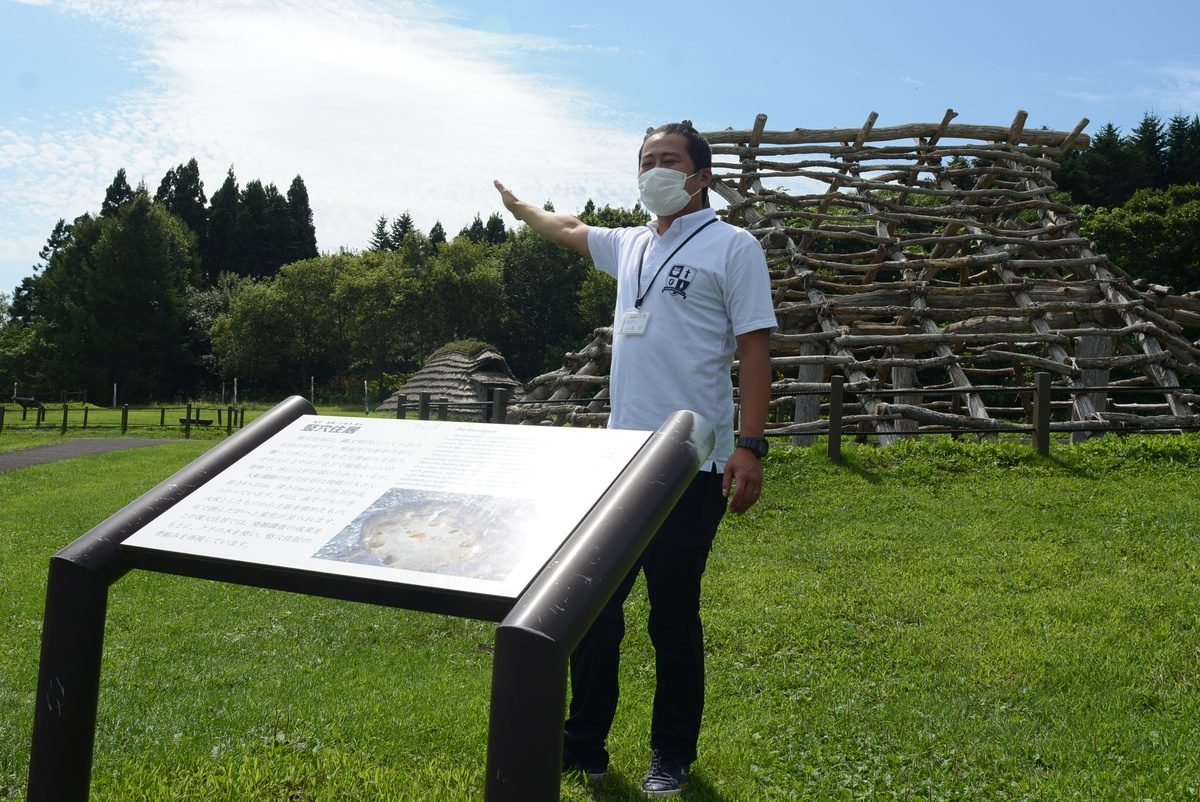
\includegraphics[width=\linewidth]{fig/01_Iseki_kengaku/02_Ofune.JPG}
	\caption{\hangindent=3zw
		120軒以上の竪穴住居跡が検出された大船遺跡の解説をする吉田会員}
	\label{}
\end{figure}

世界文化遺産の構成資産の一つである大船遺跡は、復元された竪穴住居が魅力です。120軒以上の竪穴住居跡が発見されています。吉田会員(函館市教育委員会)から解説をいただきました。

\subsection{クリ材で復元された竪穴住居}

竪穴に柱・梁・垂木を加えた復元竪穴住居です。躯体を構成する木材は、発掘調査成果を踏まえ、クリ材が使用されています。クリは北海道には自生しないと言われていますので、大船遺跡出土のクリ材はもともとは本州東北地方北部にあったものが遺跡周辺に持ち込まれたようです。吉田会員は「クリを栽培していた、とまでは言えないが、縄文時代の人たちはクリ林に対して何らかの管理を行いながら利用していたと考えられます」と述べました。

\begin{figure}[ht]
	\centering
	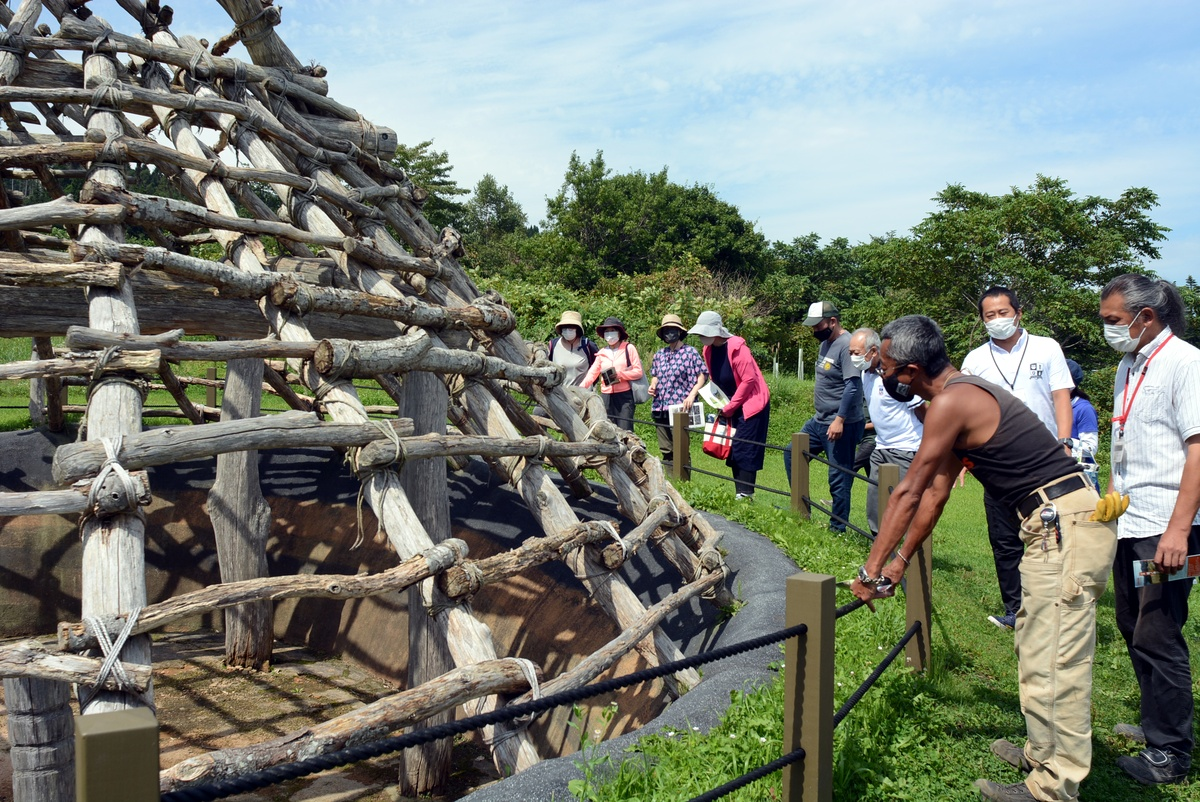
\includegraphics[width=\linewidth]{fig/01_Iseki_kengaku/04_Ofune_house.JPG}
	\caption{\hangindent=3zw
		発掘調査成果にもとづいて、クリ材で躯体を復元した竪穴住居}
	\label{}
\end{figure}

\subsection{竪穴住居の内部は20℃}

復元された竪穴住居の屋根材はカヤで葺かれています。洞爺湖町入江貝塚や岩手県御所野遺跡では土葺き屋根の復元をしていますが、大船遺跡では土葺きを積極的に肯定する資料が得られていないため茅葺きとしたそうです。

\begin{figure}[ht]
	\centering
	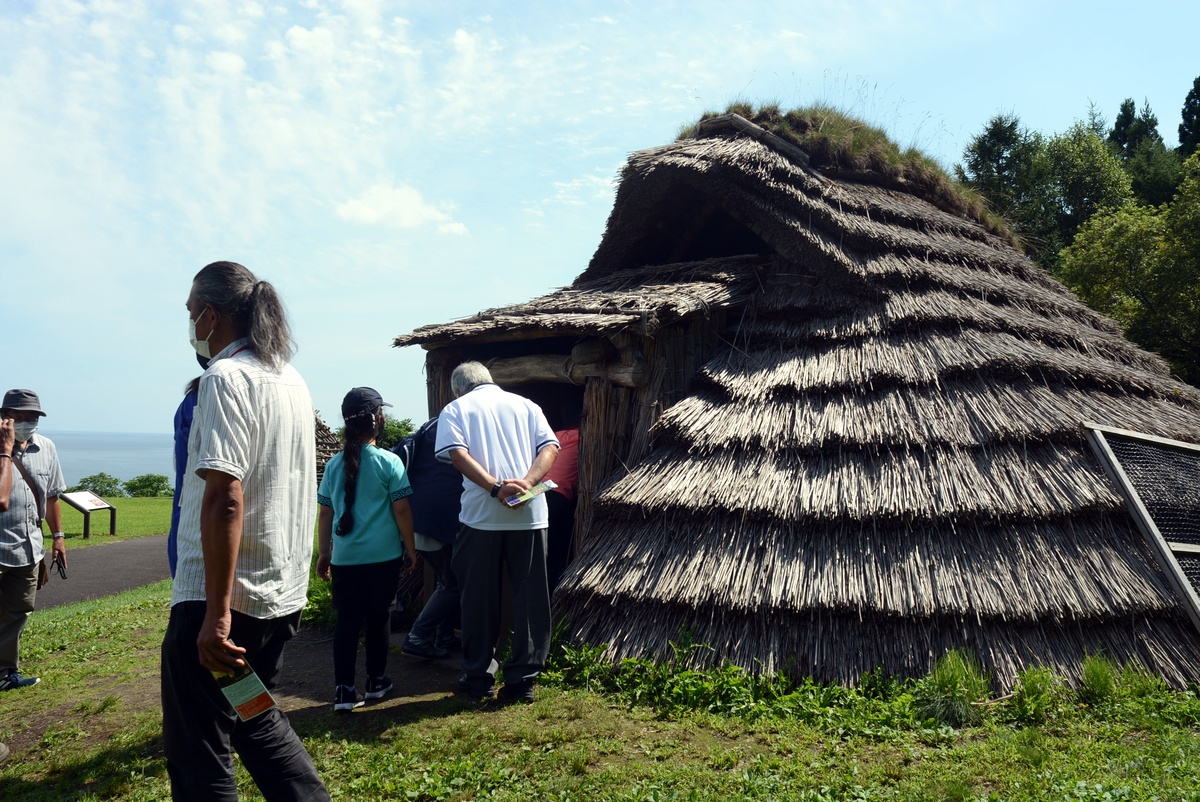
\includegraphics[width=\linewidth]{fig/01_Iseki_kengaku/06_Ofune_house.JPG}
	\caption{茅葺きの復元案を採用した竪穴住居}
	\label{}
\end{figure}

見学当日、外気温は28℃でしたが、復元住居の中は約20℃で非常に涼しい環境でした。住居内には炉が設置され、湿気抜き、明かり取りなどのために、一年を通して火を焚いていたと考えられるそうです。炉の手前にみえる小さな穴は、胎盤を埋めた穴ではないかとのことでした。

\begin{figure}[ht]
	\centering
	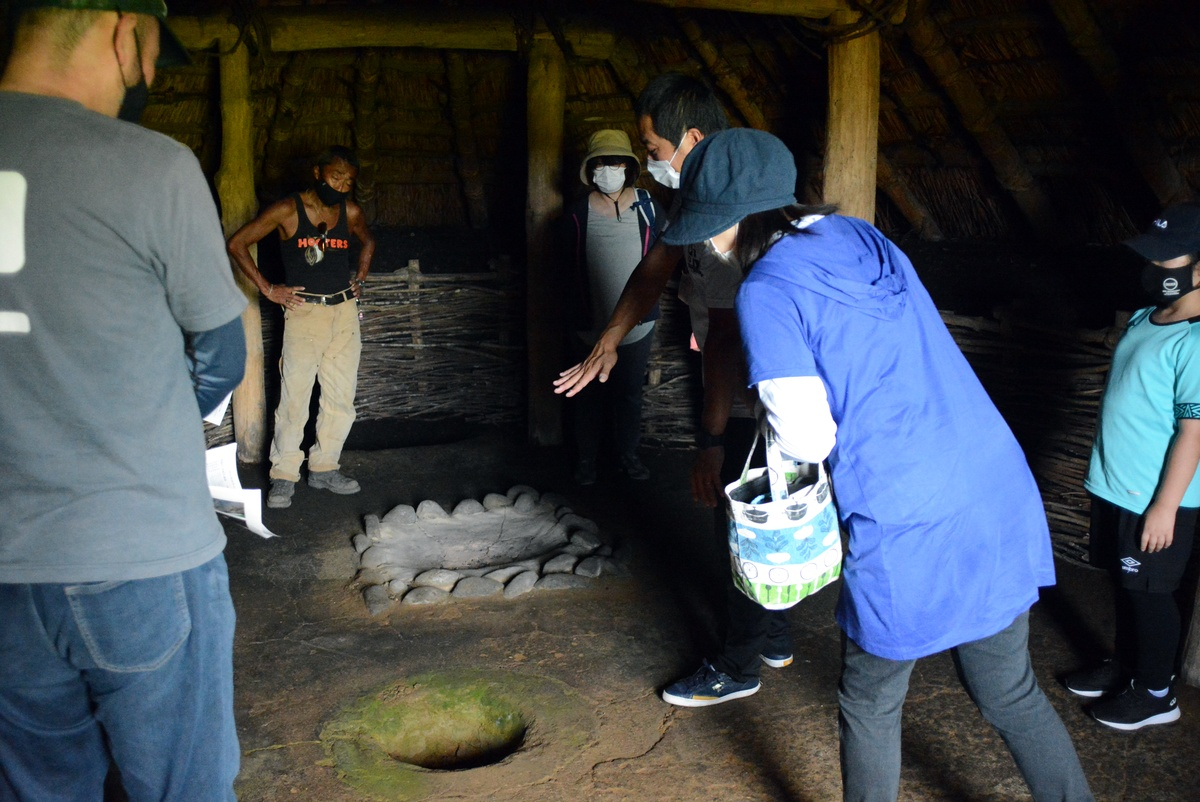
\includegraphics[width=\linewidth]{fig/01_Iseki_kengaku/07Ofune_inner_house.JPG}
	\caption{夏でも涼しい復元住居}
	\label{}
\end{figure}

%%%%
\subsection{もっとも深い竪穴は2.4m}

大船遺跡の竪穴住居は非常に深いことが特徴です。「冬寒いので深い竪穴を必要とした」という説明は、より寒さの厳しい道東や道北の竪穴住居が必ずしも深いわけではないことから成立しません。吉田会員は「火山灰層を掘り抜いて、固いローム層まで到達するためにはこのぐらいの深さが必要だったのではないか」と推測します。

\begin{figure}[ht]
	\centering
	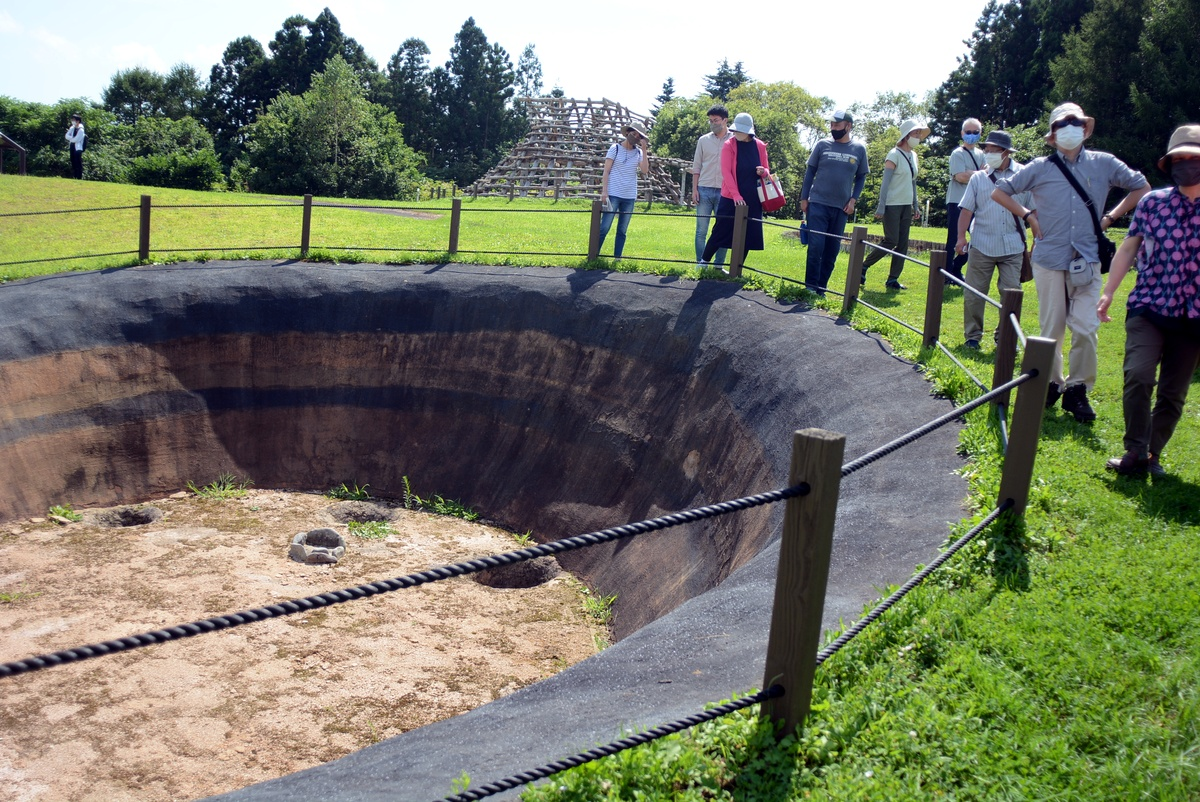
\includegraphics[width=\linewidth]{fig/01_Iseki_kengaku/08DeepHouse.JPG}
	\caption{大船遺跡を代表する深さ2.4mの竪穴住居}
	\label{}
\end{figure}

%%%%
\section{後期初頭の集落跡が見つかった大船B遺跡}

大船遺跡から少し北に進んだところに大船B遺跡があります。見学日にはすでに調査完了状態で、足の踏み場もないほど竪穴住居跡や柱穴が検出されていました。

\begin{figure}[ht]
	\centering
	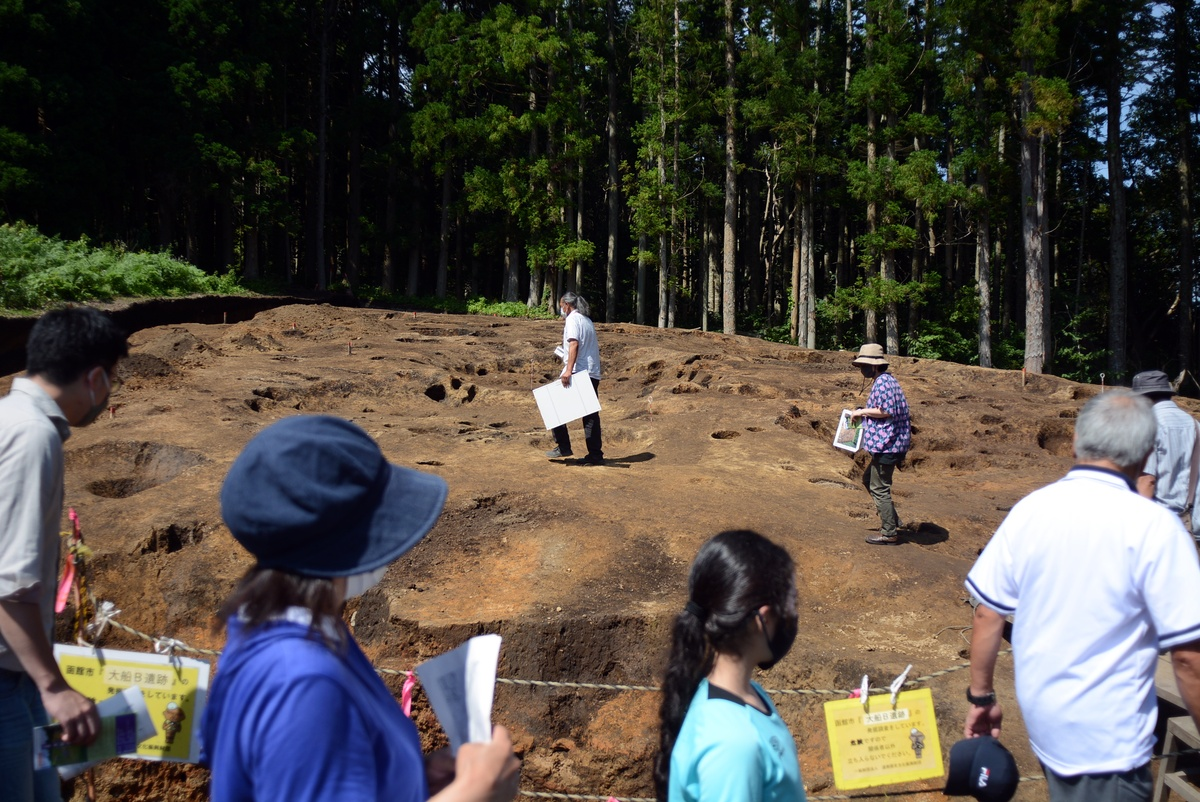
\includegraphics[width=\linewidth]{fig/01_Iseki_kengaku/09_OfuneB_zenkei.JPG}
	\caption{調査が完了したばかりの大船B遺跡}
	\label{}
\end{figure}

%%%%
\subsection{厚く堆積する火山灰}

調査担当者の荻野会員に土層断面の解説をしていただきました。上層の白い火山灰は昭和4年(1929)降灰のKo-a火山灰、その下層にKo-d(1640年)やB-Tm(923年)が見えます。

\begin{figure}[ht]
	\centering
	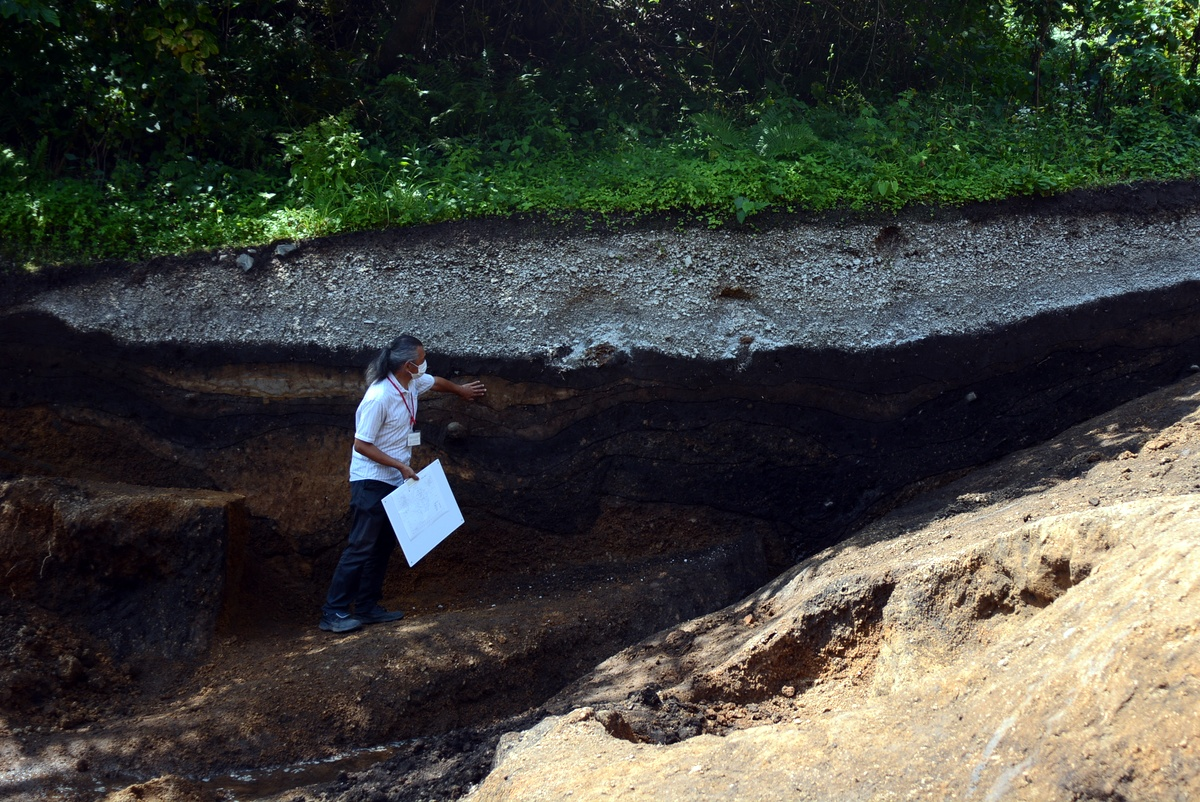
\includegraphics[width=\linewidth]{fig/01_Iseki_kengaku/10_OfuneB_section.JPG}
	\caption{大船B遺跡の土層断面}
	\label{}
\end{figure}

%%%%
\subsection{31軒検出された後期初頭の竪穴住居}

大船B遺跡で検出された竪穴住居は中期2軒、後期初頭31軒、後期後葉1軒です。後期初頭の竪穴住居は何軒も重なって構築されています。

\begin{figure}[ht]
	\centering
	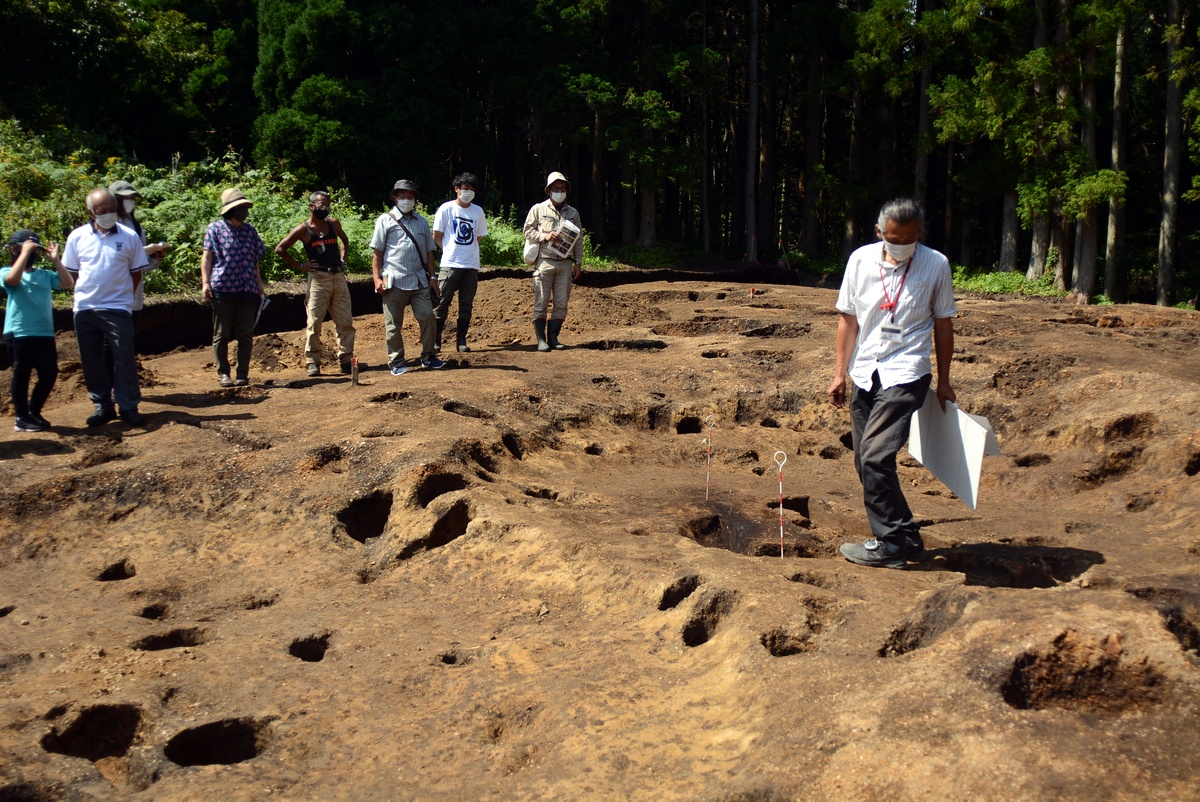
\includegraphics[width=\linewidth]{fig/01_Iseki_kengaku/11_Ofune_house.JPG}
	\caption{縄文後期の竪穴群}
	\label{}
\end{figure}

%%%%
\section{縄文時代の景観が残る垣ノ島遺跡}

垣ノ島遺跡は海岸段丘上に立地しています。現在の集落は段丘の下にありますが、遺跡からは全く見ることができません。

\begin{figure}[ht]
	\centering
	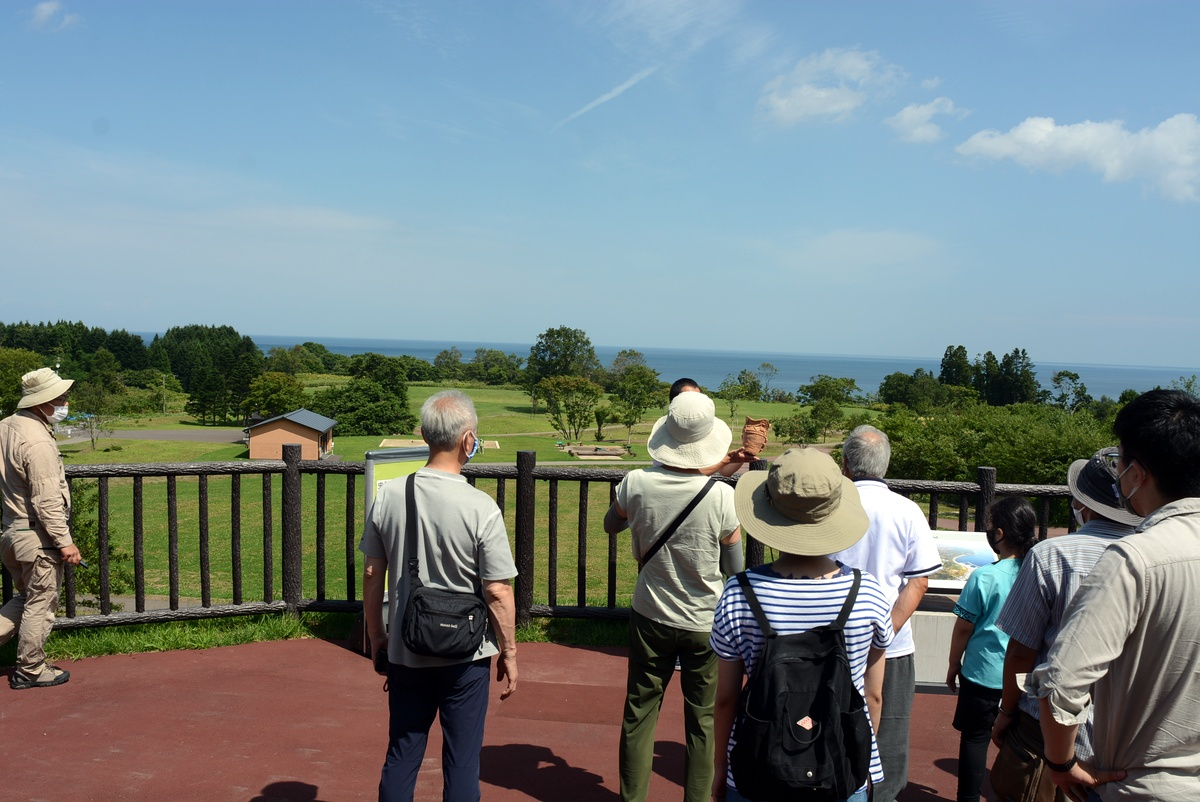
\includegraphics[width=\linewidth]{fig/01_Iseki_kengaku/12_Kakinosima_zenkei.JPG}
	\caption{\hangindent=3zw
		縄文時代と変わらない景観が広がる垣ノ島遺跡}
	\label{}
\end{figure}

%%%%
\subsection{バリアフリーな遺跡}

垣ノ島遺跡は一見平坦ですが、それなりに傾斜があります。園路はすべてスロープが設けられ、最大でも4\%以下の勾配となるように設計されていて、誰でも遺跡を楽しめる配慮がなされています。電動キックスケーターのような移動手段の導入も考えられそうです。

\begin{figure}[ht]
	\centering
	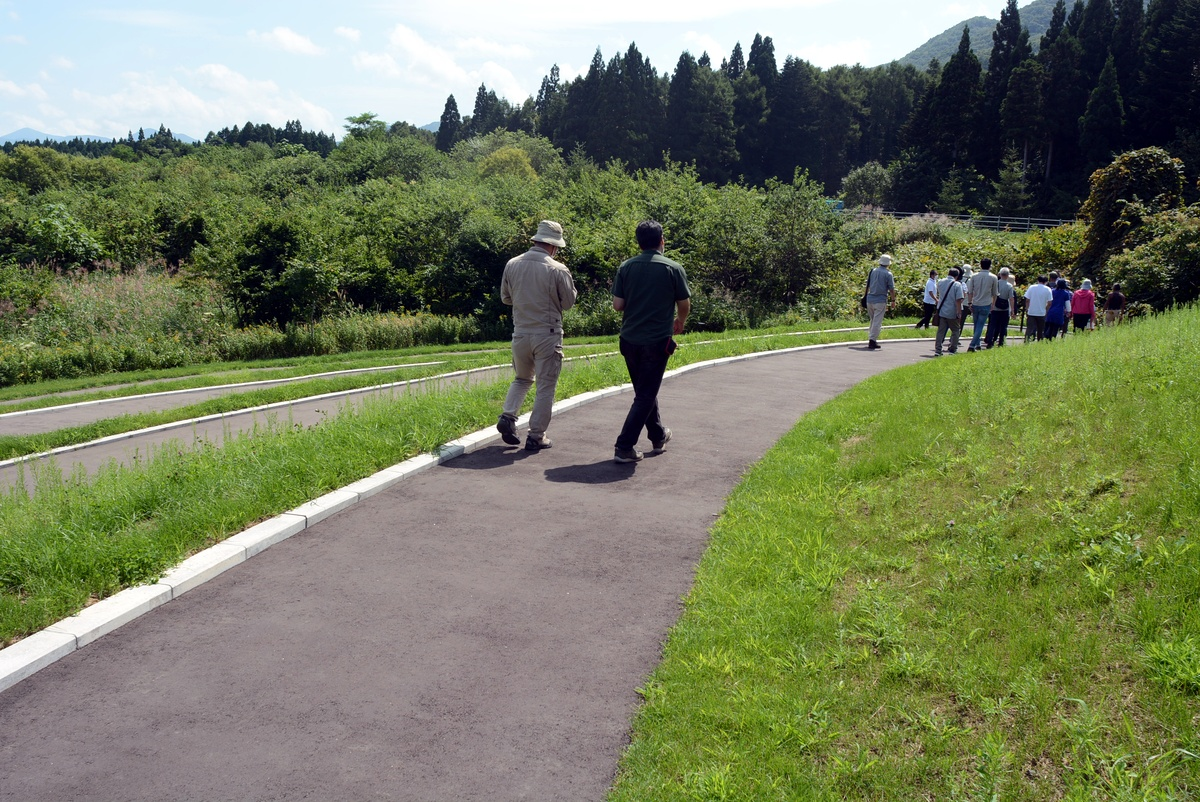
\includegraphics[width=\linewidth]{fig/01_Iseki_kengaku/13Kakinosima_slope.JPG}
	\caption{バリアフリーに配慮されたスロープ}
	\label{}
\end{figure}

%%%%
\subsection{発掘体験コーナー}

史跡の一角には発掘体験コーナーが設けられています。箕や移植ゴテ、ハケなどの発掘道具が一式用意されています。本物の土器を発見することができる魅力的なアクティビティです。

\begin{figure}[ht]
	\centering
	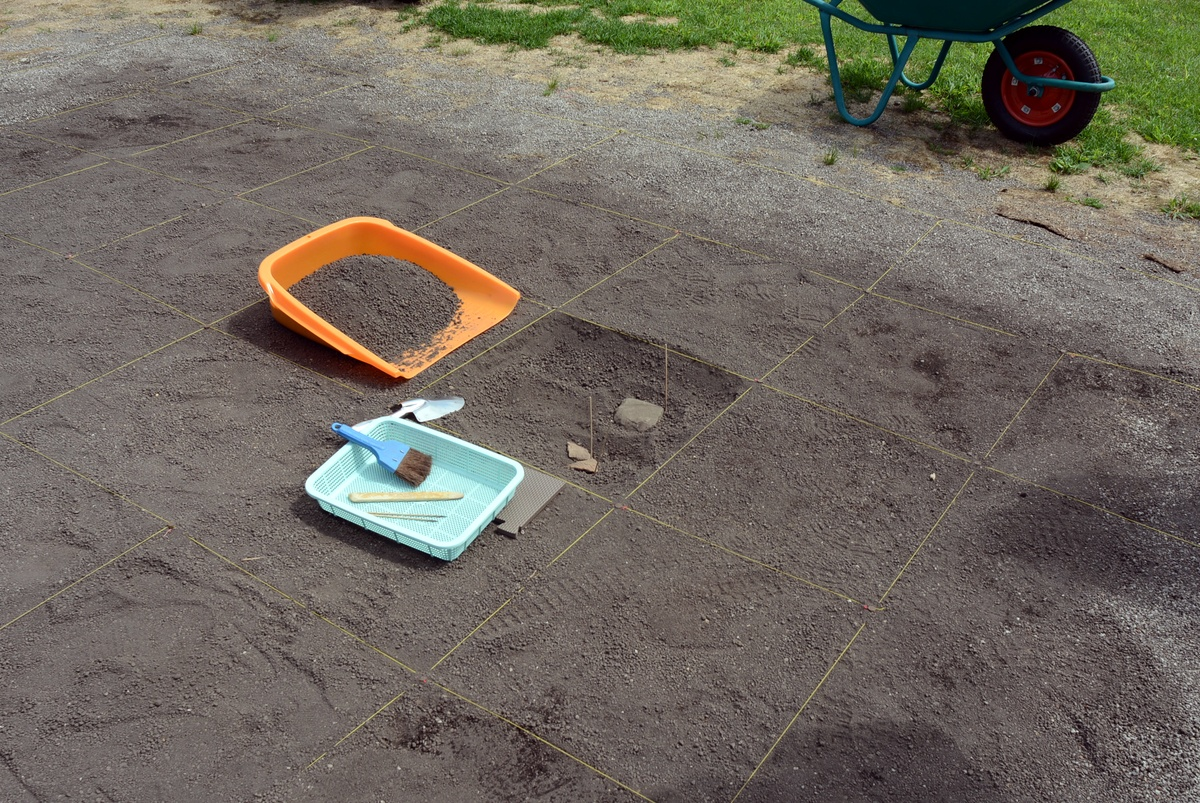
\includegraphics[width=\linewidth]{fig/01_Iseki_kengaku/14Hakkutu_taiken.JPG}
	\caption{\hangindent=3zw
		本物の縄文土器が出土する発掘体験コーナー}
	\label{}
\end{figure}

%%%%%
\subsection{地表面に残る竪穴のくぼみ}

垣ノ島遺跡では、地表面に竪穴のくぼみがわずかに残っています。整備ではこのくぼみを活かし、草刈り方法を変えることによって地表面で遺構を観察できるような配慮がなされています。

\begin{figure}[ht]
	\centering
	\includegraphics[width=\linewidth]{fig/01_Iseki_kengaku/15Kakinosima_tateana.JPG}
	\caption{刈り残しで表現した竪穴}
	\label{}
\end{figure}

%%%%
\subsection{大規模な盛土遺構}

垣ノ島遺跡の特徴は「コの字」状の大規模な盛土遺構です。火山灰が厚く堆積していることを活かして保護層を最低限とし、できるだけグラウンドレベルの変更が少ない状態で盛土遺構を観察できるよう工夫されています。

\begin{figure}[ht]
	\centering
	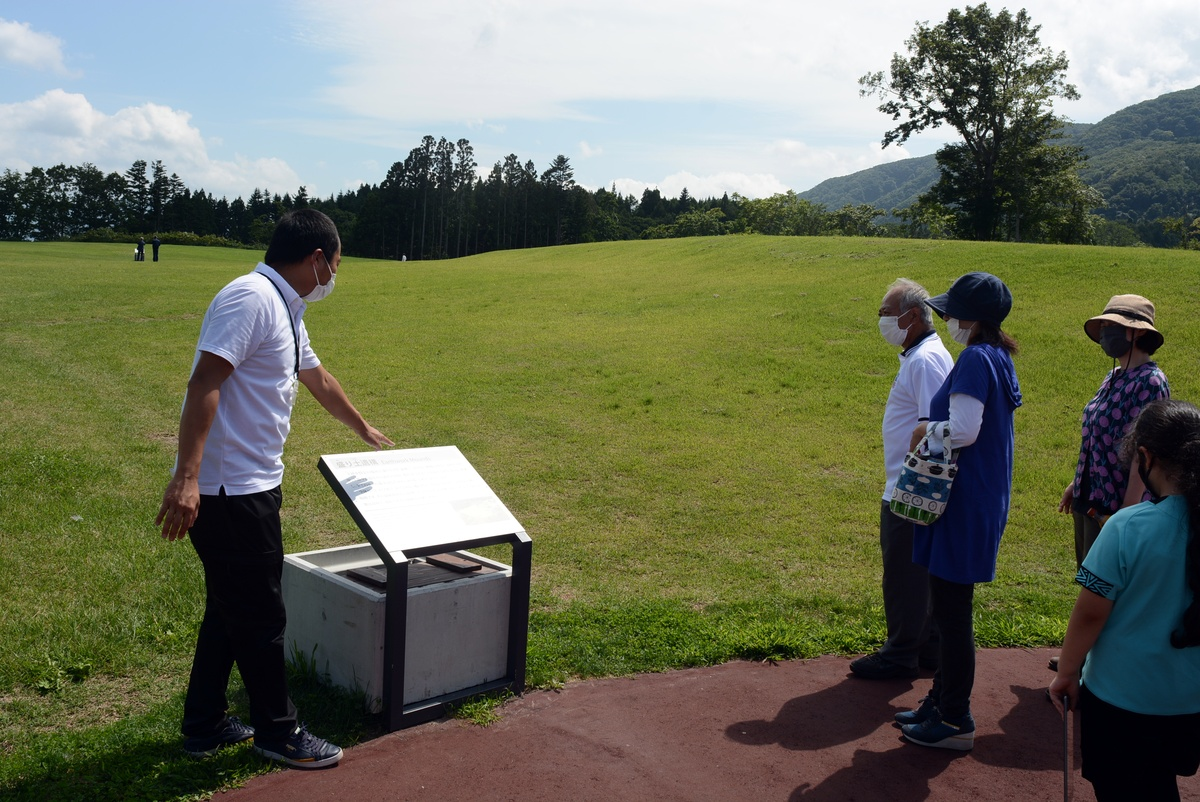
\includegraphics[width=\linewidth]{fig/01_Iseki_kengaku/16Kakinosima_morido.JPG}
	\caption{盛土遺構}
	\label{}
\end{figure}

\subsection{史跡に優しい遺構解説板}
垣ノ島遺跡で目を引くのは、基礎を打たない構造の解説板です。解説板の下部フレームの上にコンクリート製の枡を置いただけのいわゆる重力式の構造です。基礎が不要なので地下遺構への影響もなく、不自然な保護盛土も必要としません。コンクリート枡は収納スペースになっていて、中には解説用グッズが納められています。素晴らしいアイディアです。

\begin{figure}[ht]
	\centering
	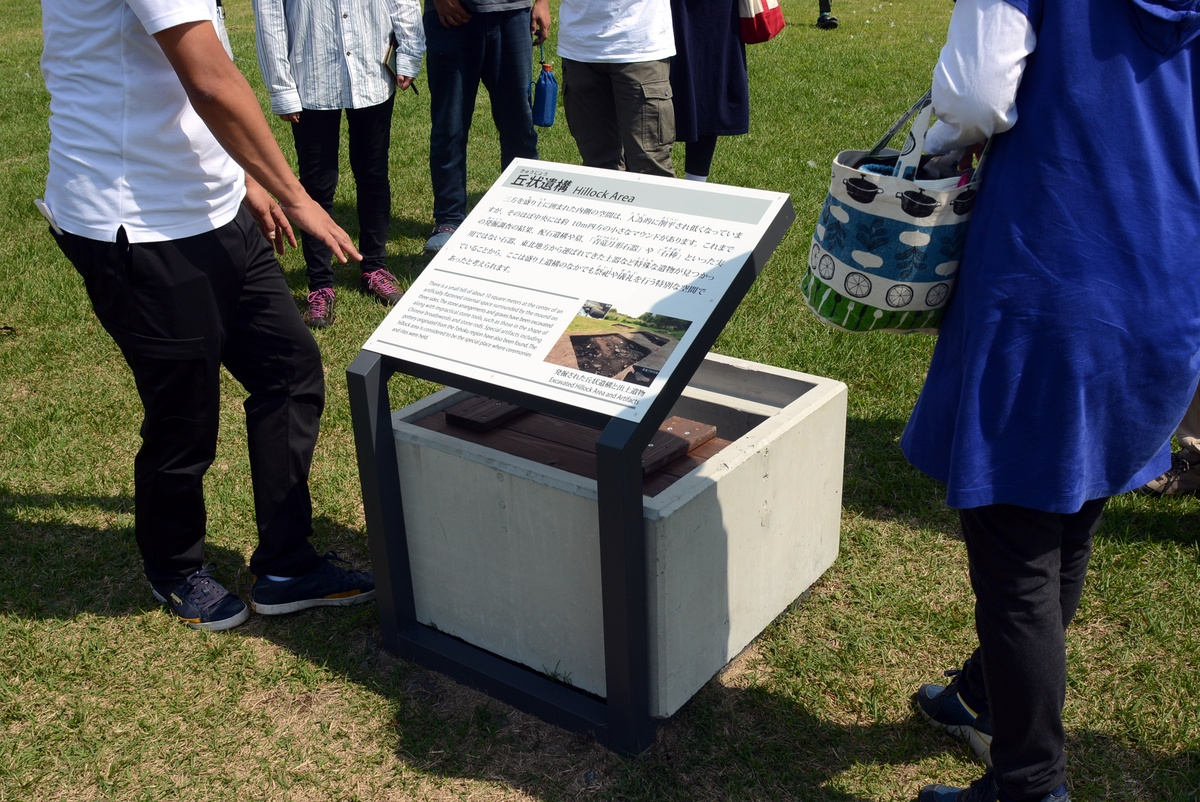
\includegraphics[width=\linewidth]{fig/01_Iseki_kengaku/17_Kakinosima_sign.JPG}
	\caption{\hangindent=3zw
		垣ノ島遺跡の解説板は地中に基礎を打たず、解説グッズ収納を兼ねたコンクリート枡で固定されています}
	\label{}
\end{figure}

%%%%
\subsection{現代構造物が全く見えないロケーション}

吉田会員は「垣ノ島遺跡は現代の構造物が全く見えない遺跡です」と強調します。舌状台地の先端から遺跡を振り返ると、史跡に関係する構造物以外、現代の構造物が何も見えません。こうしたロケーションも世界遺産の構成資産となる重要な要件だったのだと、改めて感じることができました。

\begin{figure}[ht]
	\centering
	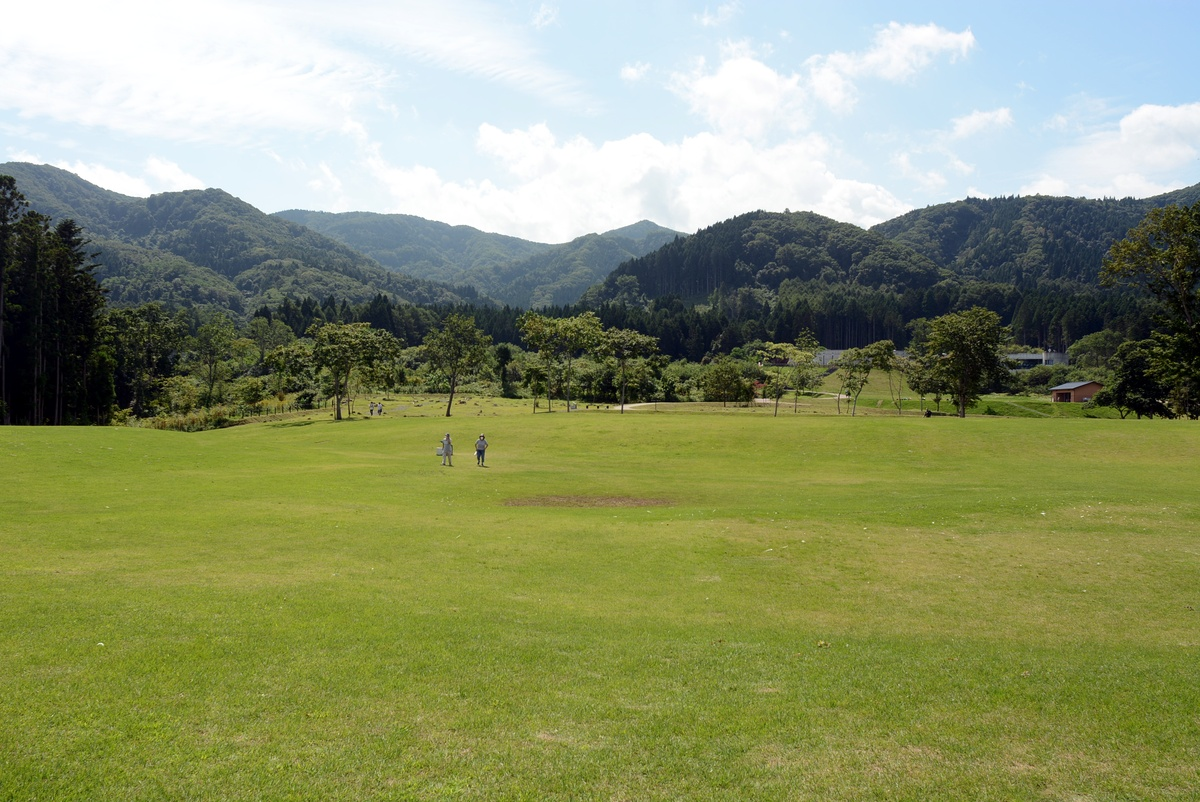
\includegraphics[width=\linewidth]{fig/01_Iseki_kengaku/18Kakinosima_zenkei02.JPG}
	\caption{\hangindent=3zw
		海岸段丘の縁から遺跡を振り返ると、ガイダンスや体験施設以外に現代の構造物が目に入りません}
	\label{}
\end{figure}

%%%%
\newpage
\section{縄文遺跡の見学を終えて}

\subsection{整備方針と遺跡の姿}
大船遺跡は視覚的にわかりやすい復元的な整備がなされています。屋根を葺いた復元住居、躯体のみ復元した住居、竪穴遺構のみを復元したものを一堂に見ることができ、発掘調査成果から復元案までの変遷を追える構成となっています。大船遺跡特有の深い竪穴住居を活かした迫力ある復元です。

一方、垣ノ島遺跡では、遺跡のオーセンティシティ(真正性)を強く意識した整備がなされていると感じます。復元的な整備が排除され、遺構そのものを見せる工夫がなされています。また、遺跡景観を非常に大切にしていることも垣ノ島遺跡の整備の特徴です。復元性の少ない遺跡は、わかりにくさをどのように克服するかが大きな課題となりますが、スタッフによる解説がこれを補うように積極的に行われ、ハードウェアに頼らず、ソフトウェアの充実によって史跡理解を深めようという狙いがあるのでしょう。

両遺跡の見学は、史跡整備における整備思想の違いや、それにともなう工夫の在り方について学ぶ機会にもなりました。

\subsection{減少する緊急調査}
大船B遺跡は、今年度道南で行われた数少ない緊急調査の一つです。かつては休みなく行われていた緊急調査が激減していることは、埋蔵文化財保護の観点からは喜ばしいことです。しかし、緊急調査の減少は、発掘調査技術の継承の難しさや新たな発見の減少にもつながりかねません。道南の発掘技術水準の維持や魅力ある考古学活動をどのように構築していくのか、緊急調査の縮小が考古学の縮小につながることのないよう、当会がその役目を果たしていく必要があると感じました。

\begin{flushright}
	(石井淳平)
\end{flushright}


%%%%
\chapter{注目の遺跡 上ノ国町洲崎館跡 }

\section{2例目の懸仏}

史跡上之国館跡のうち洲崎館跡(上ノ国町)の発掘調査で、昨年度に花沢館跡で発見された北海道初の懸仏(如意輪観音)に続き、北海道で2例目となる懸仏が出土しました。

\begin{figure}[ht]
	\centering
	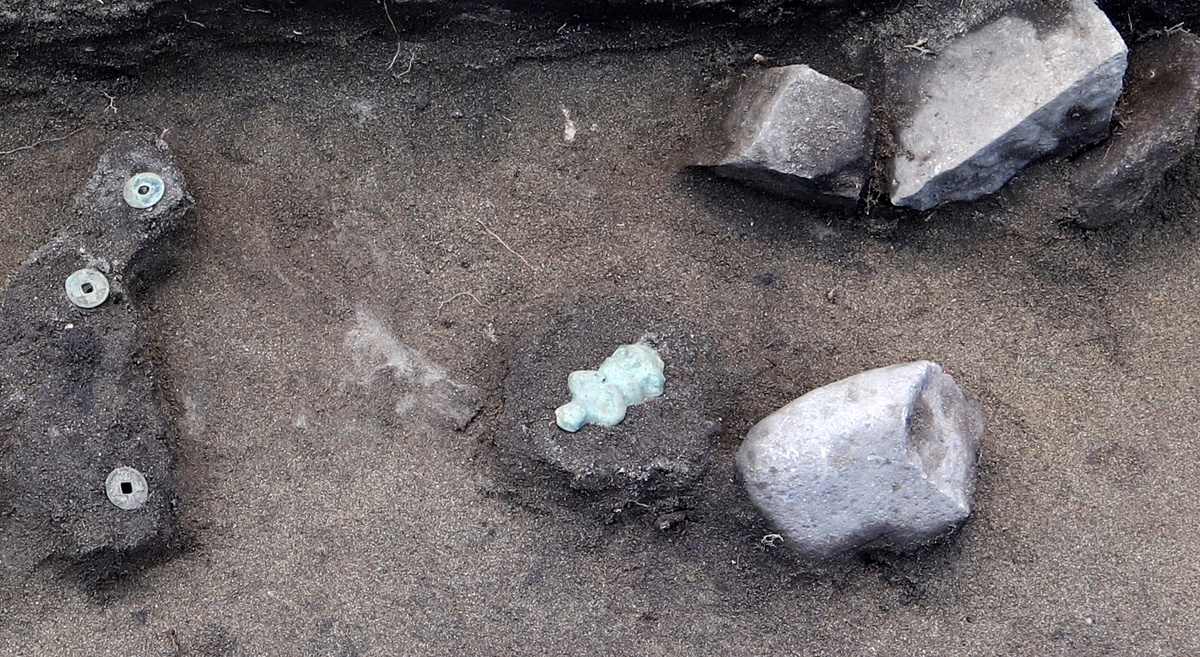
\includegraphics[width=\linewidth]{fig/08_Tukada/02shutudo.JPG}
	\caption{懸仏の出土状況}
	\label{}
	\vspace{-\baselineskip}
\end{figure}

懸仏は「御正体」(みしょうたい)とも呼ばれ、仏が仮に神の姿となって救済のため現れるという神仏習合の思想を体現し、吊るすための穴や鐶座が付いた鏡板に仏像等を線刻もしくは貼付したものです。

\section{洲崎館跡}

\begin{figure}[ht]
	\centering
	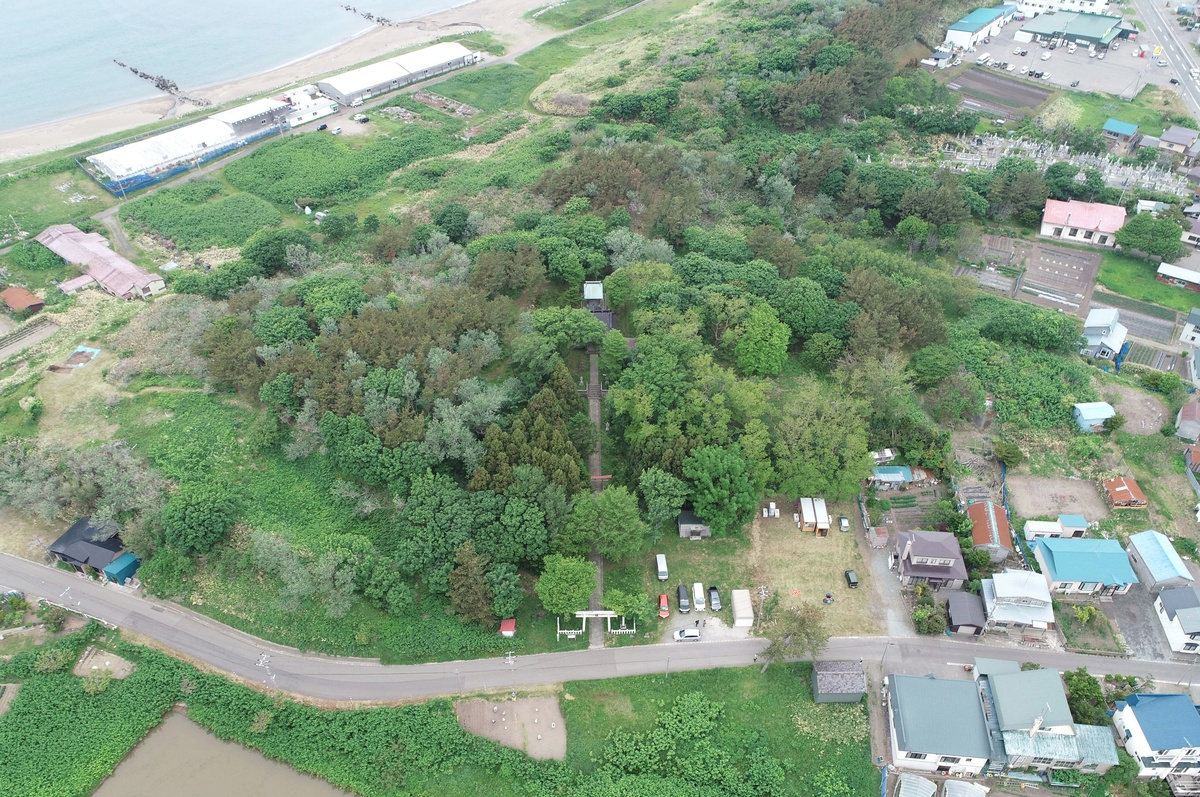
\includegraphics[width=\linewidth]{fig/08_Tukada/01enkei.JPG}
	\caption{国指定史跡洲崎館跡全景}
	\label{}
	\vspace{-\baselineskip}
\end{figure}

洲崎館跡は、長禄元年(1457)のコシャマインの戦いを収束させた武田信広によって天の川河口右岸に築かれた中世城館です。同年に信広は、蠣崎季繁の養女(下国安藤政季の娘)と結婚し、寛正3年(1462)に砂館神社の前身である、毘沙門金像を納めた毘沙門堂を建立しています(『新羅之記録』所収)。毘沙門堂は、安永7年(1778)の火災で本殿・拝殿ともに焼失し、松前藩によって翌年再建され、明治4年(1871)の神仏分離の際に砂館神社と改称しています。

\begin{figure*}[ht]
	%	\vspace{-\baselineskip}
	\centering
	\includegraphics[width=\linewidth]{fig/08_Tukada/kakebotoke.pdf}
	\caption{洲崎館跡出土の懸仏}
	\label{}
\end{figure*}


\section{北方を護る毘沙門天}
懸仏は、砂館神社西側の第3調査区で1640年降下の駒ヶ岳d火山灰(Ko-d)より下位に位置する中世の遺物包含層から出土しました。大きさは高さ8.2cm×幅4.0cm×厚1.0cmで左手の持物や鏡板は欠損していますが、甲冑を表す刻み模様や須弥山をイメージした岩座に立つ姿から毘沙門天と考えられます。懸仏の製作年代は、類例などから14\CID{00665}15世紀頃と思われ、製作技法は銅板打ち出しで、昨年度出土した鋳造の如意輪観音とは異なっています\footnote{
	大学考古学資料館2008『服部和彦氏寄贈資料図録\ajRoman{2}』)
}。
また、毘沙門天は四方を守護する四天王のうち北方を守護する「多聞天」とされ、単独で祀られる際に「毘沙門天」と呼ばれることから、今回発見された懸仏が毘沙門堂に懸けられて、蠣崎氏の北方守護の役割を担っていたことが考えられます。

\begin{flushright}
	塚田直哉(上ノ国町教育委員会)
\end{flushright}

%%%%
\chapter{会員の活動 日頃の取り組みを紹介します}

\section{ただ一人の学芸員の展示室開設までの道のり}
瀬棚町、北檜山町、大成町の3つの町が合併して生まれたせたな町は、平成29年(2017)に初めて学芸員を採用しました。せたな町は北海道指定の有形文化財「瀬棚南川の出土遺物」をはじめ、貴重な考古資料を数多く所蔵しています。初めての学芸員として赴任した工藤会員は、3つの旧町に分散した博物館資料を集成し、平成30年(2018)に北檜山区のせたな生涯学習学センターに展示室をオープンさせました。

%%%%
\subsection{せたな町教育委員会奉職まで}
私は平成26年(2014)に札幌大学大学院を卒業したのち、斜里町立知床博物館で発掘調査員として川上1遺跡、チャシコツ岬上遺跡の発掘調査及び報告書作成に従事し、翌年、白老町の仙台藩白老元陣屋資料館で臨時職員として2年間務めたのち、縁があり平成29年(2017)にせたな町で正職員の学芸員として勤めることになりました。

%%%%
\subsection{せたな町の文化財}

せたな町は北海道の南西部、日本海に面した檜山管内北部に位置しており、平成17年(2005)年9月1日に瀬棚郡瀬棚町・瀬棚郡北檜山町・久遠郡大成町の3つの町が合併し「せたな町」として新たなにスタートした町です。

\begin{figure}[H]
	\centering
	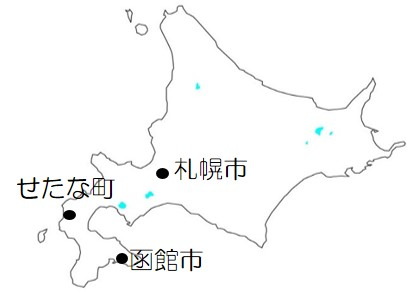
\includegraphics[width=0.8\linewidth]{fig/04_Kudo/fig01.jpg}
	\caption{せたな町の位置}
	\label{}
%	\vspace{-1\baselineskip}
\end{figure}

旧瀬棚郡北檜山町に行政の中心がおかれ、瀬棚町から町名を、久遠郡大成町から郡名を引き継ぎ、合併によって町の総面積は638,68km2と広大になっています。人口は約7,400人(令和3年8月現在)となっています。主な文化財としましては、国指定重要無形民俗文化財「松前神楽」、道指定有形文化財「南川遺跡出土の遺物」、町指定有形文化財「荻野吟子の遺品及び資料」、「青い目の人形」、「明珍信家製作の筋兜」、「阿波人形浄瑠璃」、町指定無形文化財「久遠神楽」があります。

%%%%
\newpage
\subsection{資料整備と新施設開館}
この町に来て、学芸員として一番初めに行ったことは収蔵資料台帳、埋蔵文化財包蔵地台帳、収蔵庫の確認でしたが、当町は合併前後ともに学芸員が不在だったので、収蔵資料台帳は途中までしか作られていないもの、まったく作られていないもの、埋蔵文化財包蔵地台帳は地番の記載がないものや遺跡範囲が明示されていないものがあるなど整理・作成途中で、収蔵庫も保存処理をせずにただ保管しただけの状況でした。

このような当町で学芸員の採用を決めた理由は、平成25年(2013)に廃校となった北海道瀬棚商業高等学校の校舎を改修して、郷土資料館、図書室、学童保育所を合わせた複合施設「せたな町立生涯学習センター」を平成30年(2018)10月1日に開館する計画があったからです。

\begin{figure}[H]
	\centering
	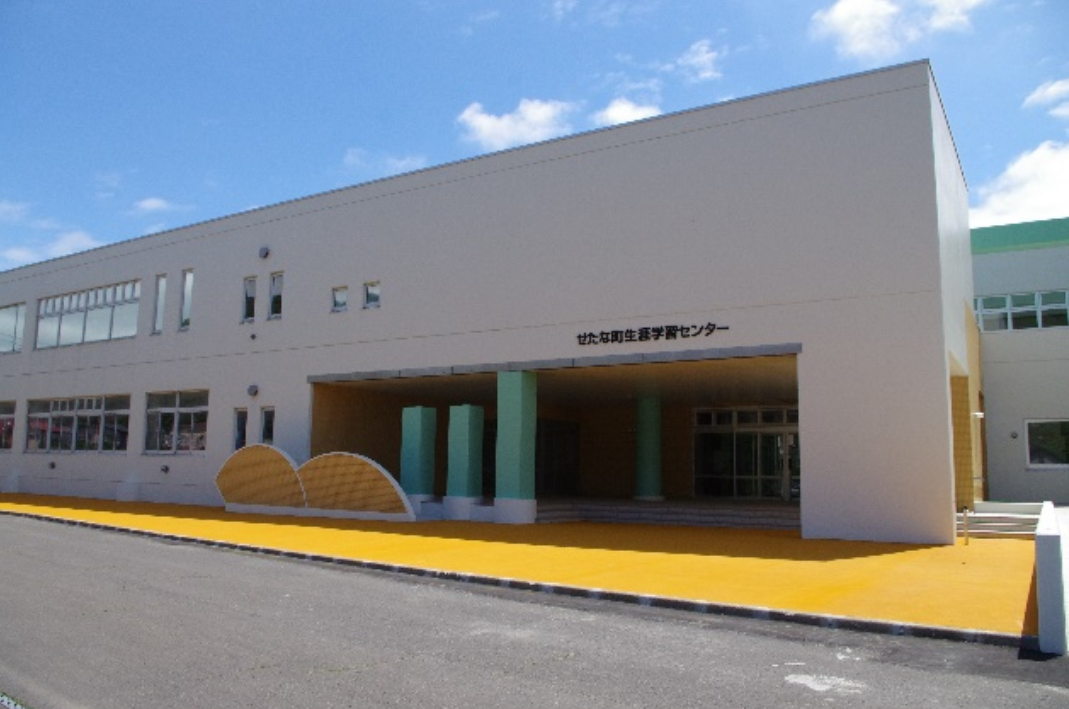
\includegraphics[width=\linewidth]{fig/04_Kudo/fig02.png}
	\caption{改修工事が終わった生涯学習センター}
	\label{}
%	\vspace{-1\baselineskip}
\end{figure}

新施設開館にあたり、展示に必要な物品リストと予算確保、収蔵資料の梱包・運搬、展示コンセプトの立案、レイアウトの作成、展示解説文の作成、展示作業、ライティングなどの開館準備と平行し、せたな町各区の歴史調査、文化財に関する普及・啓発活動として埋蔵文化財や郷土史に関する講話や体験事業、各郷土資料館における企画・特別展示の実施、埋蔵文化財保護業務などの通常の学芸業務に加え、社会教育業務や教育委員会業務もやらなければならず、小さな町の学芸員は1人で1から10までやらなければならないということを、身をもって実感しながらも平成30年(2018)10月1日に開館することができました。

\begin{figure}[H]
	\centering
	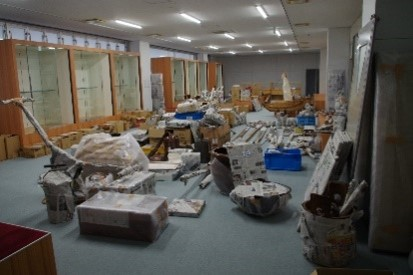
\includegraphics[width=\linewidth]{fig/04_Kudo/fig03.jpg}
	\caption{展示資料搬入状況}
	\label{}
%	\vspace{-1\baselineskip}
\end{figure}

開館して3年が経ちましたが、改善点ばかりが日々目につきます。皆さんが当町のお近くを通ることがありましたら、ぜひ足を運んで、お気づきの点などご教示いただければと思います。

\begin{figure}[H]
	\centering
	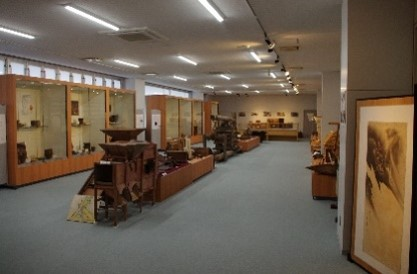
\includegraphics[width=\linewidth]{fig/04_Kudo/fig04.jpg}
	\caption{生涯学習センター展示状況}
	\label{}
\end{figure}

\begin{flushright}
工藤 大(せたな町教育委員会)
\end{flushright}

%%%%
\newpage
\section{史跡館城跡で金属探査}

明治元年(1868)に築城された館城跡で金属探査を実施しましたので、その成果の概要を報告します。

%%%%
\subsection{館城跡の礎石と御殿}
金属探査実施区域は、平成21年度の地表面調査で良好に礎石が残存していることが確認されています。これらの建物は奥御殿や常御殿と推測されており、藩主とその家族の居所や藩主が日中の政務を行う空間など、館城にとって中枢的な建物群と考えられています。また、陶磁器のほか、釘や鎹、銅製の金具などの金属製品も採集されています。これらのことから、非破壊による金属製品分布を把握することにより、館城に築かれた御殿建築の実態や空間的な機能を推測できると考えました。

%%%%
\subsection{金属探査の方法}

金属探査に使用した機材はホビー用の金属探知機(商品名「GC-1072 Metal Detector」)です。事前のテストでは、ミニエー銃弾、硬貨(1円、10円、100円)には距離10cm以内で的確に反応することを確かめています。

\begin{figure}[h]
	\centering
	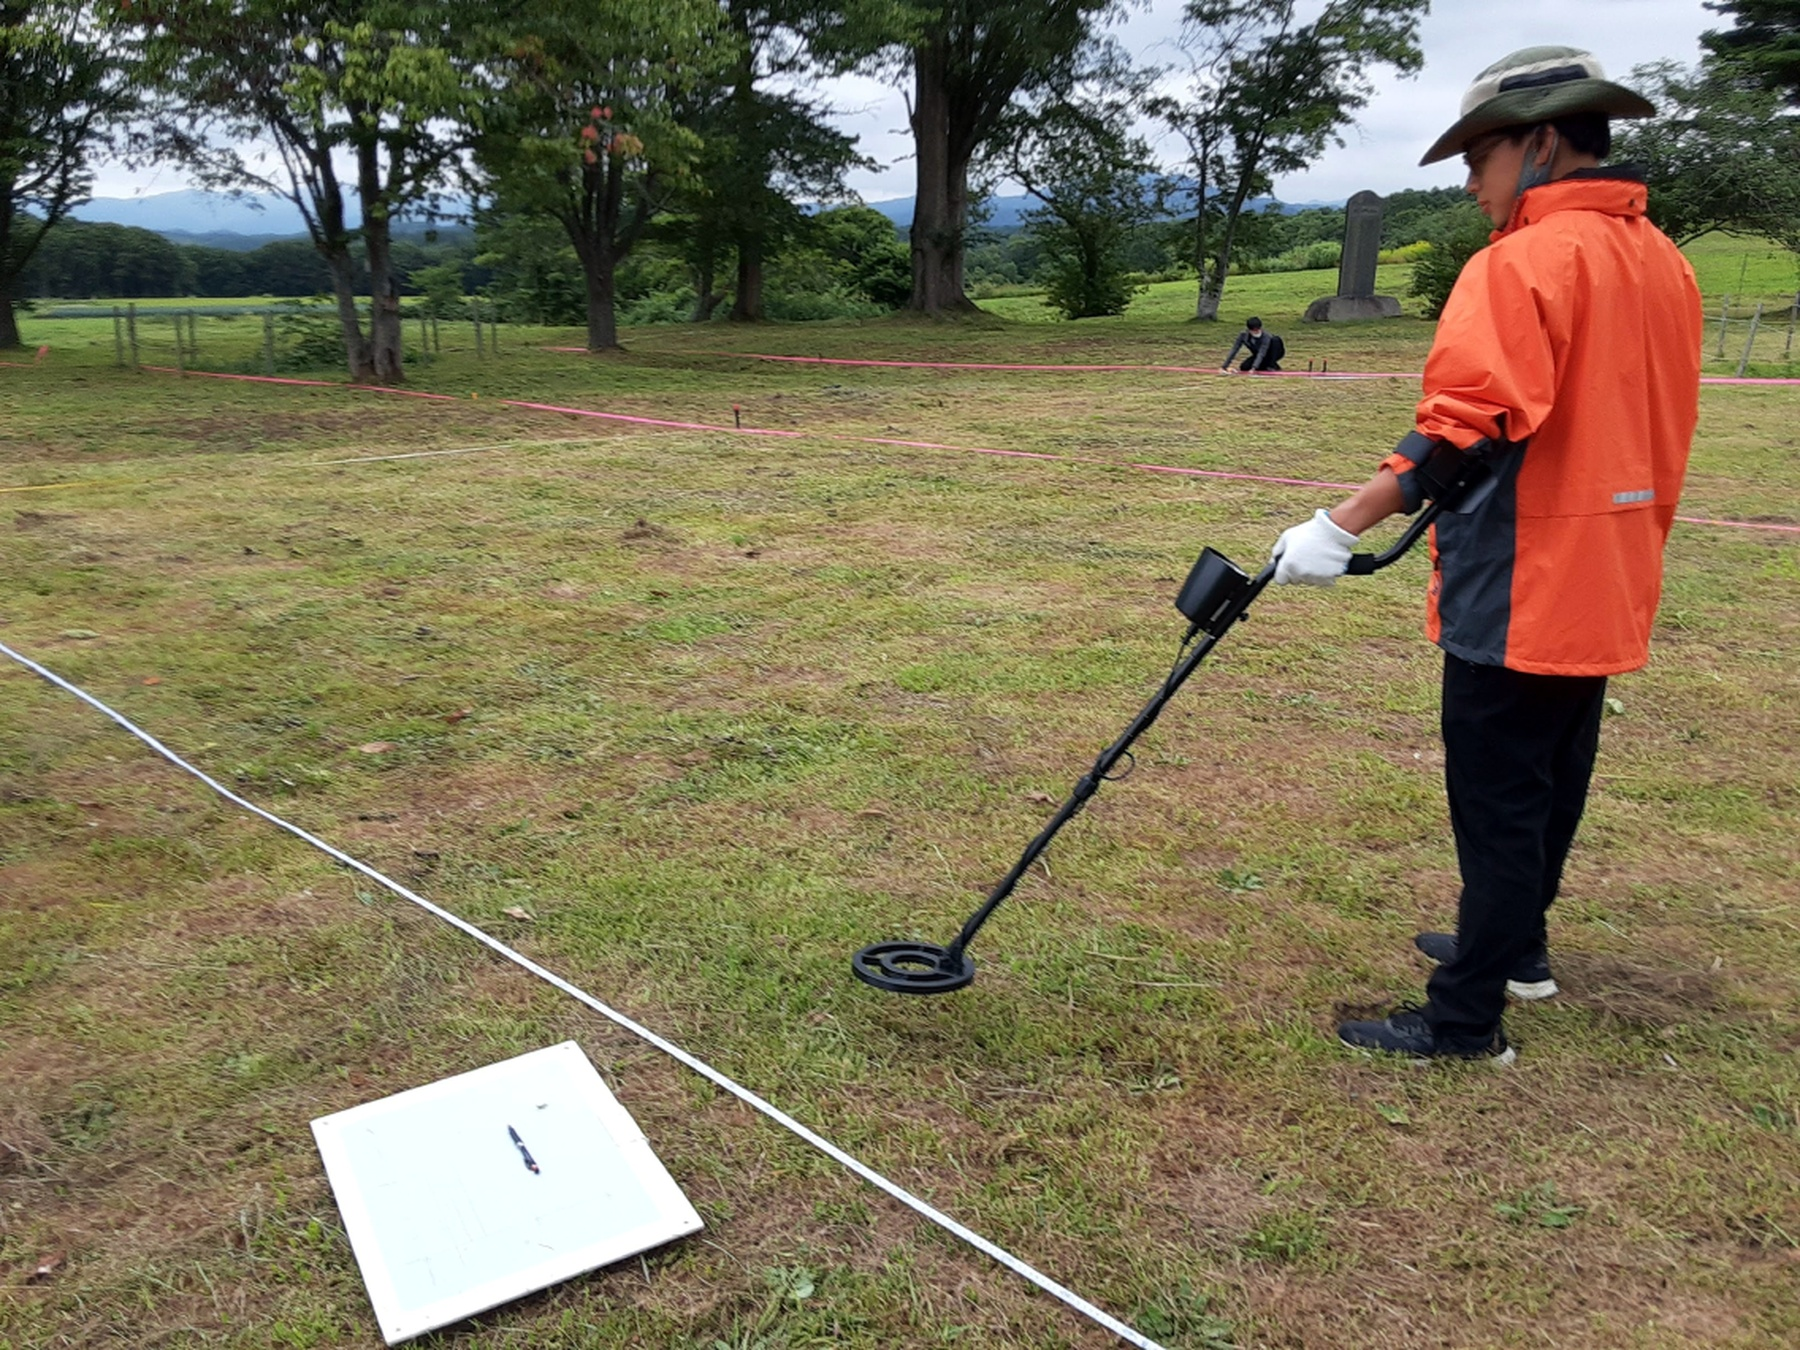
\includegraphics[width=\linewidth]{fig/07_Ishii/02survey_pic.jpg}
	\caption{金属探査実施の様子}
	\label{metal_pic}
	\vspace{-1\baselineskip}
\end{figure}

国土座標(世界測地系平面直角座標系11系)に準拠した測線を使用し、探査範囲の南北方向に測線を設定しました。測線に沿って金属探知機を移動しながら反応地点を検出しました。反応の検出においては、複数回の走査で再現性のある反応を示す地点を反応地点として記録しました。


%%%%
\subsection{金属探査の結果}

調査区の北東部、南東部、南西部の3箇所に金属反応の集中域が確認できました(図\ref{res})。調査区には礎石の配置から2棟の建物が存在すると推定されており(厚沢部町教育委員会 2010: 69)、2つの建物に挟まれたx=7730\CID{00665}7740の領域は金属反応の分布密度が低いことが読み取れます。平成21年度の礎石調査の出土遺物の分布も東側建物に多く見られることから、過去の調査結果とも整合する反応分布といえます。

\begin{figure}[ht]
	\centering
	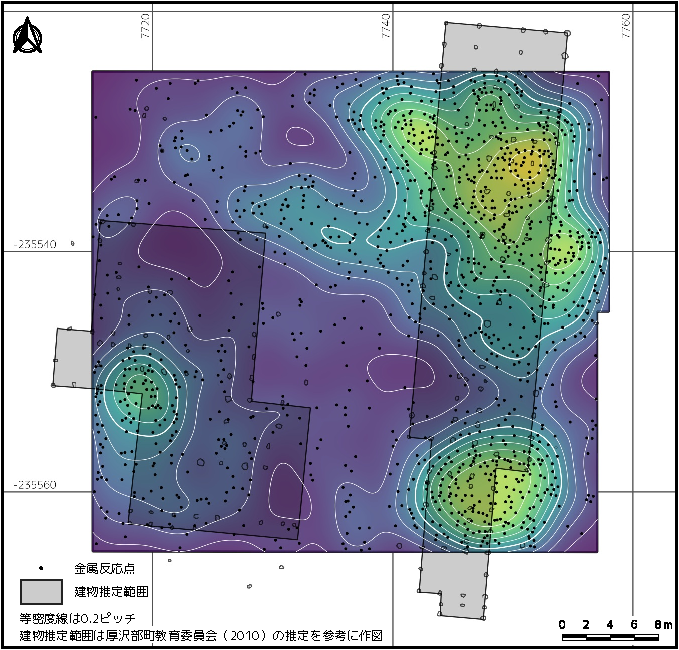
\includegraphics[width=\linewidth]{fig/07_Ishii/Metal_survey_result.pdf}
	\caption{史跡館城跡金属探査の結果}
	\label{res}
\end{figure}

%%%%
\subsection{金属探査の結果}

金属反応の分布は礎石建物の領域と合致し、館城築城時に持ち込まれた金属の集積実態を反映しているものと考えられます。本探査は館城の主要建築物である奥御殿及び常御殿において優先的に建築・整備された空間領域の存在を示唆するものと考えています。

\begin{flushright}
	(石井淳平)
\end{flushright}


%%%%
\chapter{会員の紹介 会員の活躍をお知らせします}

%%%%
\section{水中考古学の魅力(江差町教育委員会・小峰彩椰さん)}

\begin{figure}[h]
	\vspace{-1\baselineskip}
	\centering
	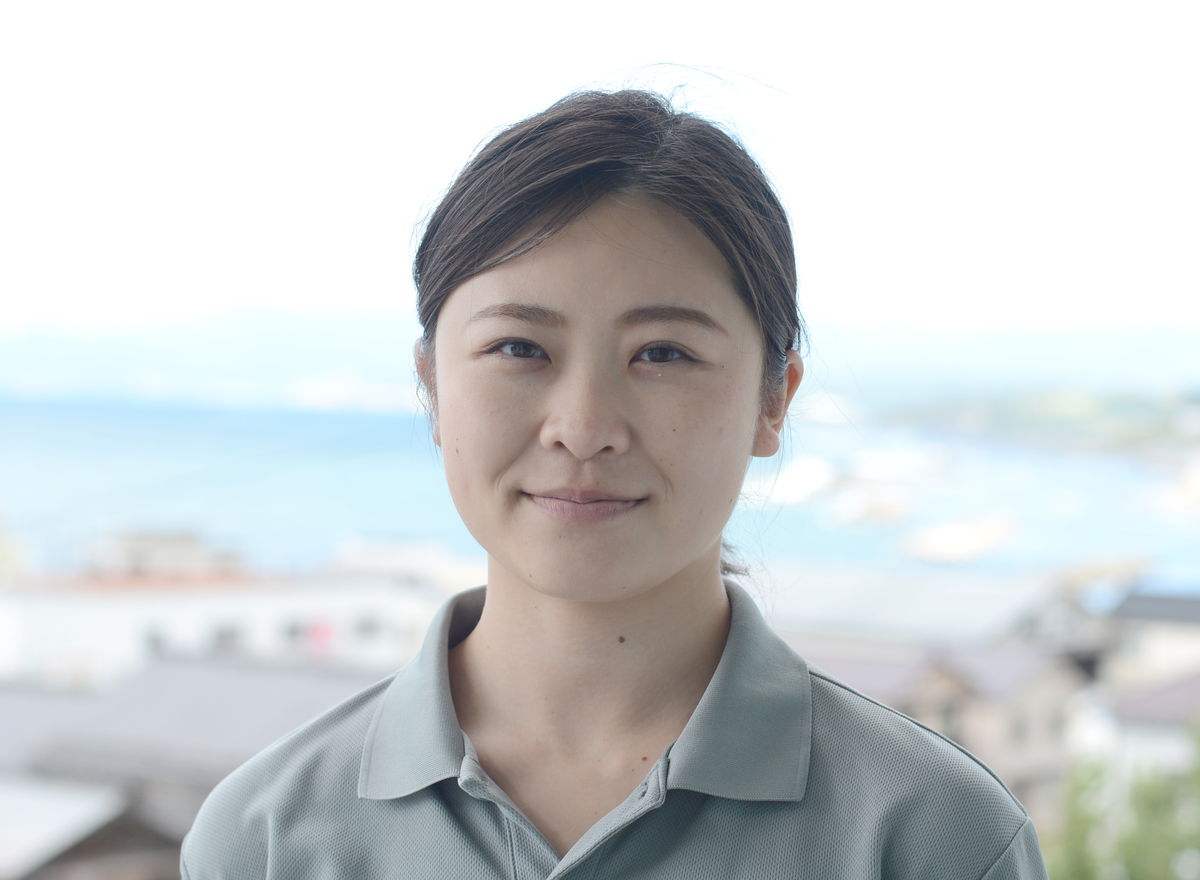
\includegraphics[width=\linewidth]{fig/02_Komine/Komine01.png}
	\caption{江差町教育委員会に配属された小峰彩椰さん}
	\label{}
%%	\vspace{-\baselineskip}
\end{figure}

小峰彩椰さんは、令和3年(2021)3月に東海大学を卒業し、同年4月に江差町教育委員会に奉職しました。専門は水中考古学です。卒業論文では、弥生時代の相模湾沿岸地域を対象とした、潟湖の地形復元と港の役割を担う遺跡の交易活動をテーマに取り上げました。

江差町では、昭和50年\CID{00665}56年に日本の水中考古学の嚆矢ともいえる開陽丸の調査が行われました。国土を海に囲まれた我が国は、海中にも多くの遺跡や遺物が眠っています。しかし、近年までその重要性が強調されることが少なかったと言えます。水中遺跡の保存に関心が持たれるようになった現在、難易度の高い水中遺跡の保護に向き合います。

現在は、博物館施設の管理運営や文化財の保護管理、開陽丸に関する文献調査を中心に行っています。開陽丸の文献調査では、オランダで行われた進水式の会食メニューの復元を試みます。

観光地である江差では町内の歴史文化に関する案内をする業務も多く、自分の知識を誰もが理解しやすい言葉で伝えることの難しさを感じていると言います。中学生を案内した際には、後日、感謝の手紙が届けられ、新しいことを知ってもらうことの嬉しさを知ったと言います

今後は自身でも郷土資料館の展示を手がけたいと考えていますが、北海道の土器型式や出土陶磁器、地域の歴史文化など、専門分野問わず勉強しなければならないことが山積しており、それらの勉強に日々取り組んでいます。また、開陽丸の発掘調査で引き揚げた遺物の保存状態には課題も多く、その改善のため、保存科学や保管方法についての知識は必須と考えています。専門領域である水中考古学についても、まだまだ知識が浅いと自評します。

\begin{figure}[ht]
	\centering
	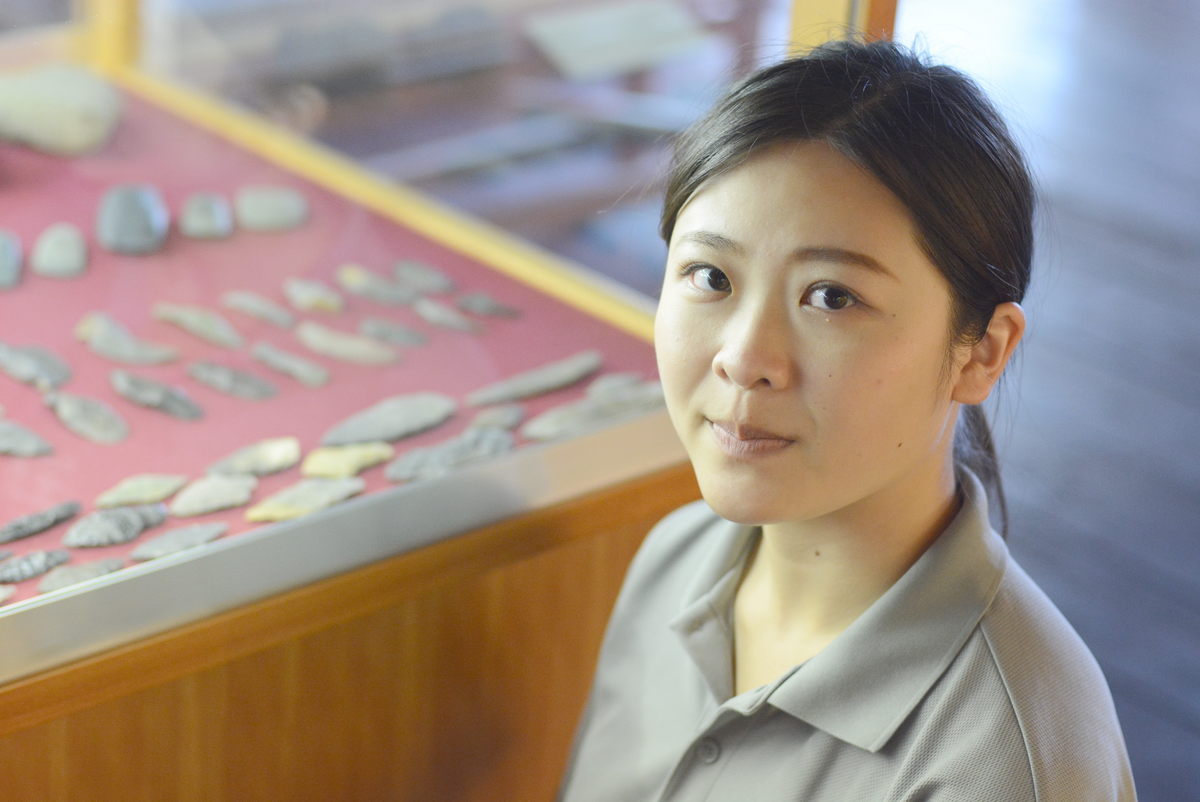
\includegraphics[width=\linewidth]{fig/02_Komine/Komine02.png}
	\caption{\hangindent=3zw
		自分でも展示を手がけてみたいが、その前にまだまだ勉強することがたくさんある、と語る小峰さん}
	\label{}
	\vspace{-1\baselineskip}
\end{figure}

当面の目標は開陽丸の保護・活用です。しかし、開陽丸が現在もなお、江差港の海底に保存されていることを知らない町民が意外にも多くいることに驚いており、町民に対する普及活動に力を入れていきたいと考えています。日本で初めて本格的に調査された水中遺跡である開陽丸の保護と活用は、日本の水中考古学の発展につながるため、各種事業や調査を精力的に行っていきたいと語ってくれました。

\hspace{8zw}(インタビュー 石井淳平)


%%%%
%\newpage
\section{中世館跡を掘る(上ノ国町教育委員会・佐藤貢平さん)}

佐藤貢平さんは、令和3年(2021)3月に札幌学院大学を卒業し、同年4月に上ノ国町教育委員会に奉職しました。現在は、塚田直哉主幹(当会事務局長)とともに史跡上ノ国館跡洲崎館の調査を進めます。

\begin{figure}[ht]
	\centering
	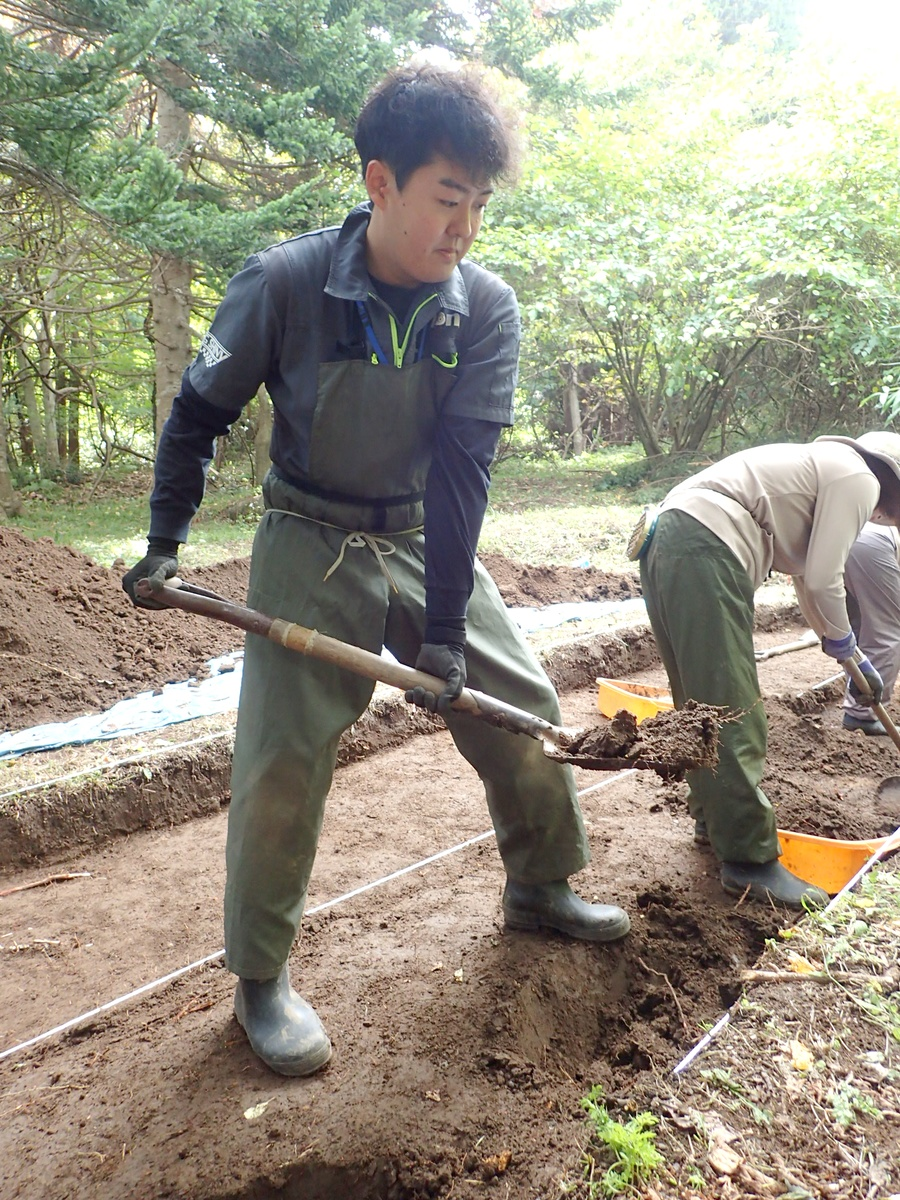
\includegraphics[width=0.9\linewidth]{fig/06_satou/s_satou.JPG}
	\caption{史跡洲崎館跡を掘る佐藤さん}
	\label{}
	\vspace{-1\baselineskip}
\end{figure}

札幌学院大学時代にはなるべく多くの現場経験を積むために、現場に参加できる機会を逃さないよう、積極的に発掘調査に参加していたと言います。発掘現場が減少している現在、発掘調査スキルを身につけるためには、自ら進んで動かなければならなかったようです。

卒業論文では現在の職場となる史跡上ノ国館跡をテーマに取り上げました。発掘調査が進められている洲崎館をはじめとし、勝山館、花沢館を含めた上ノ国の館跡の歴史的な位置づけを検討しました。そうした学生時代の経験を活かし、現在は、史跡上ノ国館跡の整備に伴う遺構確認調査に関わっています。

今年度、史跡洲崎館跡の発掘調査では花沢館跡につづく2例目の懸仏が発見されました。佐藤さん自身が担当者として関わっている遺跡から出土したことは、非常に大きな喜びだったと言います。一方、「考古学の知識が足りていないことは日々感じている」と佐藤さんは語ります。二度はできない発掘調査ですから、まずは上ノ国町内で出土する遺構や遺物について、しっかりと観察し、適切な所見が導き出せるようになりたいと考えています。

将来の目標を尋ねると「上ノ国の館跡については勿論、道南の館跡についても研究していきたい」と答えてくれました。より多くの人に上ノ国をはじめとした道南の中世について知ってもらえるように取り組んでいきたいと抱負を語ってくれました。 

\hspace{8zw}(インタビュー 石井淳平)

%%%%
\chapter{書評 プロセス考古学の第一人者、初の日本語書籍}

\begin{description}	[leftmargin=3.5zw] %ぶら下がりインデントを調節
	\item[書 名]過去を探求する\CID{00661}考古資料解読の方法と実践\CID{00661}
	\item[刊 行]2021年6月10日
	\item[編著者]ルイス・R・ビンフォード
	\item[発 行]株式会社雄山閣
\end{description}

\begin{figure}[H]
	\centering
	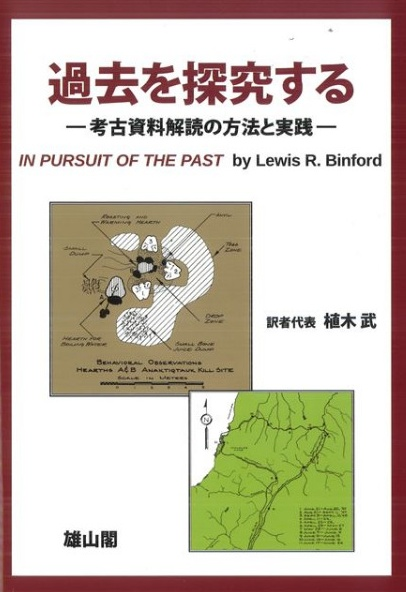
\includegraphics[width=0.8\linewidth]{fig/09_Shohyo/Binford.jpg}
%	\caption{}
	\label{}
%	\vspace{-\baselineskip}
\end{figure}

プロセス考古学の第一人者ルイス・ビンフォード教授の著作のうち、日本語で読める唯一の単著です。ビンフォードはV.G.チャイルドやI.ホッダーなどと並んで日本で最も知名度の高い海外考古学者でしょう。チャイルドやホッダーの著書は数十年前から日本語訳されていましたが、ビンフォードの著作は長く日本語化されることはありませんでした。本書は考古学ファンにとって待望の一冊といえます。

本書はビンフォードが目ざした「遺構・遺物に意味を与える理論的な道具」の開発について理解するための最良の書です。1980年から1981年にかけて行われた講演・講義記録を中心に成り立っているため、話し言葉をベースとした本書は、翻訳陣の努力もあり、初学者にも読みやすい平易な文体で書かれています。

ページの多くはアフリカや北米の狩猟採集民の観察に費やされています。まるで民族誌の研究書のようですが、観察された考古資料から自然の営為によるものと人間の活動の結果によるものを区分し、それぞれの形成過程を考察していきます。大量の考古資料について観察を積み重ねれば自ずと過去の人間活動が見えてくると信じる旧世代の考古学の限界を、多くの実例によって指摘します

「モノに始まりモノに終わる」のが考古学ではない、というビンフォードの声が本書のいたるところから聞こえるように感じました。\\
\hspace{15zw}(石井淳平)



\end{document}
